\documentclass[final, 12pt]{colt2018} % Anonymized submission
% \documentclass{colt2017} % Include author names

% The following packages will be automatically loaded:
% amsmath, amssymb, natbib, graphicx, url, algorithm2e

\usepackage{times}
\usepackage{epstopdf}
%\usepackage{subcaption}
%\newcommand{\mc}{\frac{\partial c_n(s_n)}{\partial s_n}}
%\newcommand{\pb}{p(\mathbf{b})}
%\newcommand{\qc}{\frac{\partial Q_n(b_n; \mathbf{b}_{-n})}{b_n}}
%\newcommand{\mz}{\frac{\partial c_n(z)}{\partial z}}
\newcommand{\norm}[1]{\left\lVert #1 \right\rVert}
\newcommand{\cost}{\mathrm{cost}}
\newcommand{\sumt}{\sum_{t=1}^T}
\newcommand{\todo}[1]{{\color{red}(TODO: #1)}}
\usepackage{etoolbox}

\ifcsmacro{theorem}{}{
\newtheorem{theorem}{Theorem}
\newtheorem{corollary}[theorem]{Corollary}
\newtheorem{lemma}[theorem]{Lemma}
\newtheorem{proposition}[theorem]{Proposition}
\newtheorem{assumption}[assumption]{Assumption}
\newtheorem{definition}[definition]{Definition}
\newtheorem{algorithm}[algorithm]{Algorithm}
\newtheorem{example}{Example}
\newtheorem{remark}{Remark}
}



\newtheorem{innercustomgeneric}{\customgenericname}
\providecommand{\customgenericname}{}
\newcommand{\newcustomtheorem}[2]{%
  \newenvironment{#1}[1]
  {%
   \renewcommand\customgenericname{#2}%
   \renewcommand\theinnercustomgeneric{##1}%
   \innercustomgeneric
  }
  {\endinnercustomgeneric}
}

\newcustomtheorem{customthm}{Theorem}
\newcustomtheorem{customlemma}{Lemma}


\usepackage{algorithm}
\usepackage{algorithmic}
\usepackage{color}
\DeclareMathOperator*{\argmin}{arg\!min}

\newcommand{\ouralg}{Online Balanced Descent}
\newcommand{\ourack}{OBD}


\usepackage{comment}
\usepackage{ifthen}
\newboolean{showcomments}
\setboolean{showcomments}{true}
\newcommand{\niangjun}[1]{  \ifthenelse{\boolean{showcomments}}
{ \textcolor{red}{(Niangjun:  #1)}} {}  }
\newcommand{\adam}[1]{  \ifthenelse{\boolean{showcomments}}
{ \textcolor{red}{(Adam:  #1)}} {}  }
\newcommand{\gautam}[1]{  \ifthenelse{\boolean{showcomments}}
{ \textcolor{red}{(Gautam:  #1)}} {}  }
\newcommand{\addcites}[0]{  \ifthenelse{\boolean{showcomments}}
{ \textcolor{red}{(Add citation(s))}} {}  }
\newcommand{\addcite}[0]{  \ifthenelse{\boolean{showcomments}}
{ \textcolor{red}{(Add citation(s))}} {}  }

\graphicspath{{figures/}}
 % Use \Name{Author Name} to specify the name.
 % If the surname contains spaces, enclose the surname
 % in braces, e.g. \Name{John {Smith Jones}} similarly
 % if the name has a "von" part, e.g \Name{Jane {de Winter}}.
 % If the first letter in the forenames is a diacritic
 % enclose the diacritic in braces, e.g. \Name{{\'E}louise Smith}

 % Two authors with the same address
  % \coltauthor{\Name{Author Name1} \Email{abc@sample.com}\and
  %  \Name{Author Name2} \Email{xyz@sample.com}\\
  %  \addr Address}

 % Three or more authors with the same address:
  \coltauthor{\Name{Niangjun Chen} $^a$\thanks{Niangjun Chen and Gautam Goel contributed equally to this work.}
  \Email{chennj@ihpc.a-star.edu.sg}\\
  \Name{Gautam Goel} $^b$\footnotemark[1] \Email{ggoel@caltech.edu}\\
  \Name{Adam Wierman} $^b$\Email{adamw@caltech.edu}\\
  \addr{$^a$ Institute of High Performance Computing} \mbox{}\hfill \addr{$^b$ California Institute of Technology}
  }
  
    
 



%\documentclass[11pt]{amsart}
%\usepackage{geometry}                % See geometry.pdf to learn the layout options. There are lots.
%\geometry{letterpaper}                   % ... or a4paper or a5paper or ... 
%%\geometry{landscape}                % Activate for for rotated page geometry
%%\usepackage[parfill]{parskip}    % Activate to begin paragraphs with an empty line rather than an indent
%\usepackage{graphicx}
%\usepackage{amssymb}
%\usepackage{epstopdf}
%\DeclareGraphicsRule{.tif}{png}{.png}{`convert #1 `dirname #1`/`basename #1 .tif`.png}
%%\newcommand{\mc}{\frac{\partial c_n(s_n)}{\partial s_n}}
%\newcommand{\pb}{p(\mathbf{b})}
%\newcommand{\qc}{\frac{\partial Q_n(b_n; \mathbf{b}_{-n})}{b_n}}
%\newcommand{\mz}{\frac{\partial c_n(z)}{\partial z}}
\newcommand{\norm}[1]{\left\lVert #1 \right\rVert}
\newcommand{\cost}{\mathrm{cost}}
\newcommand{\sumt}{\sum_{t=1}^T}
\newcommand{\todo}[1]{{\color{red}(TODO: #1)}}
\usepackage{etoolbox}

\ifcsmacro{theorem}{}{
\newtheorem{theorem}{Theorem}
\newtheorem{corollary}[theorem]{Corollary}
\newtheorem{lemma}[theorem]{Lemma}
\newtheorem{proposition}[theorem]{Proposition}
\newtheorem{assumption}[assumption]{Assumption}
\newtheorem{definition}[definition]{Definition}
\newtheorem{algorithm}[algorithm]{Algorithm}
\newtheorem{example}{Example}
\newtheorem{remark}{Remark}
}



\newtheorem{innercustomgeneric}{\customgenericname}
\providecommand{\customgenericname}{}
\newcommand{\newcustomtheorem}[2]{%
  \newenvironment{#1}[1]
  {%
   \renewcommand\customgenericname{#2}%
   \renewcommand\theinnercustomgeneric{##1}%
   \innercustomgeneric
  }
  {\endinnercustomgeneric}
}

\newcustomtheorem{customthm}{Theorem}
\newcustomtheorem{customlemma}{Lemma}


\usepackage{algorithm}
\usepackage{algorithmic}
\usepackage{color}
\DeclareMathOperator*{\argmin}{arg\!min}

\newcommand{\ouralg}{Online Balanced Descent}
\newcommand{\ourack}{OBD}


\usepackage{comment}
\usepackage{ifthen}
\newboolean{showcomments}
\setboolean{showcomments}{true}
\newcommand{\niangjun}[1]{  \ifthenelse{\boolean{showcomments}}
{ \textcolor{red}{(Niangjun:  #1)}} {}  }
\newcommand{\adam}[1]{  \ifthenelse{\boolean{showcomments}}
{ \textcolor{red}{(Adam:  #1)}} {}  }
\newcommand{\gautam}[1]{  \ifthenelse{\boolean{showcomments}}
{ \textcolor{red}{(Gautam:  #1)}} {}  }
\newcommand{\addcites}[0]{  \ifthenelse{\boolean{showcomments}}
{ \textcolor{red}{(Add citation(s))}} {}  }
\newcommand{\addcite}[0]{  \ifthenelse{\boolean{showcomments}}
{ \textcolor{red}{(Add citation(s))}} {}  }

\title{ Smoothed Online Convex Optimization in High Dimensions  \quad \\ via Online Balanced Descent}
%\author{The Author}
%\date{}                                           % Activate to display a given date or no date

\begin{document}
\maketitle



\begin{abstract}
We present preconditioned stochastic gradient descent (SGD) algorithms for the $\ell_1$ minimization problem $\min_{\xx}\|\AA \xx - \bb\|_1$ in the overdetermined case, where there are far more constraints than variables. Specifically, we have $\AA \in \R^{n \times d}$ for $n \gg d$. Commonly known as the Least Absolute Deviations problem, $\ell_1$ regression can be used to solve many important combinatorial problems, such as minimum cut and shortest path. SGD-based algorithms are appealing for their simplicity and practical efficiency.
% Our algorithms precondition the matrix $\AA$ and then solve the problem for the resulting matrix $\tilde{\AA}$ using gradient descent techniques.
Our primary insight is that careful preprocessing can yield preconditioned matrices $\tilde{\AA}$ with strong properties (besides good condition number and low-dimension) that allow for faster convergence of gradient descent. In particular, we precondition using Lewis weights to obtain an isotropic matrix with fewer rows and strong upper bounds on all row norms. We leverage these conditions to find a good initialization, which we use along with recent smoothing reductions and accelerated stochastic gradient descent algorithms to achieve $\epsilon$ relative error in $\Otil(nnz(\AA) + d^{2.5} \epsilon^{-2})$ time with high probability, where $nnz(\AA)$ is the number of non-zeros in $\AA$. This improves over the previous best result using gradient descent for $\ell_1$ regression. We also match the best known running times for interior point methods in several settings.

Finally, we also show that if our original matrix $\AA$ is approximately isotropic and the row norms are approximately equal, we can give an algorithm that avoids using fast matrix multiplication and obtains a running time of $\Otil(nnz(\AA) + s d^{1.5}\epsilon^{-2} + d^2\epsilon^{-2})$, where $s$ is the maximum number of non-zeros in a row of $\AA$. In this setting, we beat the best interior point methods for certain parameter regimes.


%We consider the $\ell_1$ minimization problem $\min_{\xx}||\AA \xx - \bb||_1$ in the overconstrained case, where there are far more constraints than variables. More specifically, we have $\AA \in \R^{n \times d}$ for $n \gg d$. By using Lewis Weights preconditioning on $\AA$ and a careful initialization, we show that a standard stochastic gradient descent algorithm achieves $\epsilon$ relative error in about $nnz(\AA) +  d^3\epsilon^{-2}$ time with high probability. If we leverage smoothing reductions in \cite{AllenZhuH16} and the accelerated stochastic gradient descent algorithms in \cite{AllenZhu17}, we can achieve a running time of about $nnz(\AA) + d^{2.5}\epsilon^{-2}$ with the same guarantees. Both of these running times improve over the previous results in \cite{YangCRM16} and the latter result is comparable to the best known running times for interior point methods \cite{LeeS15}.
%
%The key idea will be to use our preconditioning to restrict our consideration to matrices $\AA$ such that $\AA^T\AA = \II$ and every row norm of $\AA$ is upper bounded by $O(\sqrt{d/n})$. \cite{cohenpeng} show that sampling $\AA$ with Lewis weights takes about $nnz(\AA) +d^{\omega}$ time and approximately preserves the minimization problem. Moreover, we can assume $n\le O(d\epsilon^{-2}\log n)$ for the sampled matrix. We then prove that all leverage scores of the sampled matrix are approximately equal. Since rotations preserve leverage scores, we can then rotate our sampled matrix to ensure that our desired properties are met in about $d^{\omega}\epsilon^{-2}$ time.
%
%Finally, we also show that if our original matrix $\AA$ is such that $\AA^T\AA \approx \II$ and the row norms of $\AA$ are bounded, we can avoid using fast matrix multiplication and prove a running time of about $nnz(\AA) + s d^{1.5}\epsilon^{-2}$, where $s$ is the maximum number of non-zeros in a row of $\AA$.

%Consequently, we will be able to restrict our consideration to matrices $A$ such that $A^TA \approx I$, and all row norms are equal, which is to say $||A_{i,:}||_2 = \sqrt{\frac{d}{n}}$ for all $i$.
%
%With a careful choice of our initial $x$, we show that standard gradient descent and stochastic gradient descent algorithms under these further assumptions only require $O(\frac{d}{\epsilon^2})$ and $O(\frac{d^2}{\epsilon^2})$ iterations, respectively, to achieve $\epsilon$ relative error with respect to the minimum objective value. Accordingly, these methods each achieve respective total runtime of $O(\frac{md}{\epsilon^2})$ and $O(\frac{d^3}{\epsilon^2})$, along with an $O(m)$ preconditioning cost, improving over the previous results in \cite{MahoneySGD}.
%
%We further examine the consequences of our assumptions when combined with smoothing reductions in [cite] and accelerated gradient descent techniques in [cite,cite]. As a result we are able to further improve the running times to $O(\frac{md}{\epsilon})$ and $O(dn\log{1/\epsilon} + \frac{d^2\sqrt{n}}{\epsilon})$.
%
%Random sampling $d\epsilon^{-2}\log{d}$ rows of $A$ will only incur error $\epsilon$ and reduces the latter running time to $O(\frac{d^{2.5}\log{d}}{\epsilon^2})$, which is then comparable to interior point methods of [cite]

\end{abstract}
%\section{}
%\subsection{}

\section{Introduction}
\label{sec: introduction}
% !TEX root = onlinevarinancebandits.tex

\section{Introduction}
% Structure:
% \begin{itemize}
% \item The approach of (Regularized) ERM and its importance in Machine Learning.
% Solving such problems with sequential optimization algorithms such as SGD/SVRG/Online K-means.
% Maybe focus on SGD as a running example.
% \item  Mentioned the alternative option is uniform sampling. Describe/illustrate how importance sampling can be used to improve the performance. Give references. 
% \item Describe how the variance of the estimates is a natural measure of performance in this setting. Mention that low variance translates to better performance, e.g. for SGD. 
% \textbf{Online Problem:}
% Similarly to  Duchi/EPFL  we formulate importance sampling an online convex optimization problem.
% Describe the approaches of Duchi/EPFL say very nice things about them give them credit and discuss the limitations of their results/approaches.
% \item State our result. State our contributions+ discuss the improvements over previous work: \\
% (i) tighter regret guarantees with respect to the simplex.\\
% (ii) Showing that regret minimization makes sense in this setting.\\
% (iii) (Hopefully) complementary lower bounds. \\
% (iii) Efficient experimental implementation showing the benefits of the proposed method
% \kl{This is for COLT, for ArXiv put the experiments in (ii) place}

% Discuss the technical challenges of our work, specifically the fact that the costs are unbounded + the bandit feedback.
% Discuss the new regularization that we introduce, its benefits (closed form formula for the FTRL) + the challenge.
% Mention other settings with unbounded losses, e.g. log loss in portfolio selection.
 
%  \textbf{Related work}
%  Who should we cite? Look at Jaggi/Duchi/EPFL for references.

% \kl{Mention (where?) that we can use our approach for coordinate descent.}

% \end{itemize}
%Among the most important paradigms in machine learning is Empirical Risk Minimization (ERM) , which is often the strategy of choice due to its generality and statistical efficiency.
Empirical risk minimization (ERM) is among the most important paradigms in machine learning, and  is often the strategy of choice due to its generality and statistical efficiency.
In ERM, we draw a set of  samples $\D=\{x_1,\ldots,x_n\}\subset \X$ from the underlying data distribution, and we aim to find a solution $w\in\W$ that minimizes the empirical risk,  %The empirical risk serves as a proxy to the expected loss which is often. 
%the objective is to  find a solution $w\in\W$ that minimizes the empirical risk based on a collection of $n$ samples $\D=\{x_1,\ldots,x_n\}\subset \X $:
\begin{equation} \label{eq:ERM}
  \min_{w\in\W }L(w) := \frac{1}{n}  \sum_{i=1}^n \ell (x_i, w),
\end{equation}
where $\ell: \mathcal{X} \times \W \rightarrow \reals$ is a given loss function, and $\W\subseteq \reals^d$ is usually a compact domain.

In this work we are interested in sequential procedures for minimizing the ERM objective, and relate to such methods as \emph{ERM solvers}.
More concretely, we focus on the regime where the number of samples $n$ is very large,  and it is therefore desirable to employ ERM solvers that only require  few passes over the dataset. There exists a rich arsenal of such efficient solvers which have been investigated throughout the years, with the canonical example from this category being  Stochastic Gradient Descent (SGD).


% among are SVRG \citep{johnson2013accelerating} and SAGA \citep{defazio2014saga},
%
%
% such efficient sequential solvers have been developed throughout the years, with the canonical example from this category being  Stochastic Gradient Descent (SGD).

Typically, such methods  require an unbiased estimate of the loss function at each round, which is usually  generated   by sampling a few points uniformly at random from the dataset.
However, by employing uniform sampling, these methods are insensitive to the intrinsic structure of the data. In case of SGD, for example, some data points might produce large gradients, but they are nevertheless assigned the same probability of being sampled as any other point. This ignorance often results in high-variance estimates, which is likely to degrade the performance.

The above issue can be mended by employing non-uniform importance sampling.
And indeed, we have recently witnessed several  techniques to do so: %techniques.
%In recent years several approaches have been developed in order to address this issue.
\citet{zhao2015stochastic} and similarly \citet{needell2014stochastic}, suggest using prior knowledge on the gradients of each data point in order to devise predefined importance sampling distributions.  \citet{NIPS2017_7025} devise adaptive sampling techniques guided by a robust optimization approach. These are only a few examples of a larger body of work 
 \citep{bouchard2015online, alain2015variance, csiba2016importance}.

Interestingly, the recent works of \cite{pmlr-v70-namkoong17a} and \cite{salehi2017} formulate the task of devising importance sampling distributions as an online learning problem with bandit feedback. In this context, they  think of the algorithm, which adaptively chooses the distribution, as a player that competes against the ERM solver. The goal of the player is to minimize the cumulative variance of the resulting (gradient) estimates.  Curiously, both methods rely on some form of the ``linearization trick''\footnote{ By ``linearization trick'' we mean that these methods update according to a first order approximation  of the costs rather than the costs themselves.} 
%\footnote{If $g_t$ is a subgradient of the convex function $f:S\rightarrow \mathbb{R}$ at $w_t$, then $f(w_t) - f(u) \leq (w_t-u)^\intercal g_t$,  $\forall u \in S$.} 
 to resort to the analysis of the EXP3  \citep{auer2002nonstochastic}.

On the other hand, the theoretical guarantees of the above methods are somewhat limited. Strictly speaking, none of them provides regret guarantees with respect to the best fixed distribution in hindsight:  \citet{pmlr-v70-namkoong17a} only compete with the best distribution among a \emph{subset} of the simplex (around the uniform distribution).  Conversely, \cite{salehi2017} compete against a solution which might perform worse than the best in hindsight up to a multiplicative factor of $3$.

In this work, we adopt the above mentioned online learning formulation, and design novel importance sampling techniques. 
Our adaptive sampling procedure is simple and efficient, and 
in contrast to previous work, we are able to provide regret guarantees with respect to the best fixed point among the simplex.
As our contribution, we
\vspace{-1.5mm}
\begin{itemize}
\setlength\itemsep{0.05em}
\item motivate theoretically why regret minimization is meaningful in this setting, 
\item propose a novel bandit algorithm for variance reduction ensuring regret  of~$\tO(n^{1/3}T^{2/3})$,
\item empirically validate our method, and provide an efficient implementation\footnote{The source code is available at  \url{https://github.com/zalanborsos/online-variance-reduction}}.
\end{itemize}
On the technical side, we do not rely on a ``linearization trick'' but rather directly employ a scheme based on the classical 
 Follow-the-Regularized-Leader approach. 
Our analysis entails several technical challenges, most notably handling  unbounded cost functions while only receiving partial (bandit) feedback. Our design and analysis draws inspiration from the seminal works of  \citet{auer2002nonstochastic}  and 
\cite{Abernethy08}. 
Although we present our method for choosing \emph{data points}, it naturally applies to choosing \emph{coordinates in coordinate descent} or even \emph{blocks} of thereof \citep{allen2016even,perekrestenko2017faster, nesterov2012efficiency, necoara2011random}.
More broadly, the proposed algorithm can be incorporated in \emph{any sequential algorithm} that relies on an unbiased estimation of the loss. A prominent  application of our method is variance reduction for SGD, which can be achieved by considering  gradient norms as  losses, i.e., replacing $\ell(w,x_i) \leftrightarrow \|\nabla \ell(w,x_i)\|$. With this modification, our method is minimizing the cumulative variance of the gradients throughout the optimization process.

%defining the bandit feedback as the norm of the gradient estimate. 
The paper is organized as follows. In Section \ref{sec:Motivation}, we formalize the online learning setup of variance reduction, and motivate why regret is a suitable performance measure. As the first step of our analysis, we investigate the full information setting in Section \ref{sec:full-info}, which serves as a mean for studying the bandit setting in Section \ref{sec:bandit}. Finally, we validate our method empirically, and provide the detailed discussion of the results in Appendix  \ref{sec:experiments}. 



%We achieve this by relying on classical results from Follow-the-Regularized-Leader framework, where the regularizer is chosen to suit the setting of variance reduction with importance sampling.

%\newpage
%
%
% rely on solving a a ro
%
%There exists
%
%In 
%Addressing the regime where the number of samples $n$ is very large, efficient \emph{sequential} procedures have been developed, that perform only a few passes over the dataset. These methods usually require an unbiased estimate of the loss function at each round, and they generate the estimate by sampling a few points uniformly at random from the dataset. The canonical example from this category is Stochastic Gradient Descent (SGD).
%
%However, by employing uniform sampling, these methods are agnostic to the intrinsic structure of the data. In case of SGD, for example, some data points might produce large gradients, but they are nevertheless assigned the same probability of being sampled as any other point. This ignorance often results in high-variance estimates.
%
%References:
%\begin{itemize}
%\item \textbf{Variance reduction with uniform sampling}: SVRG \citep{johnson2013accelerating} and SAGA \citep{defazio2014saga}, \cite{xiao2014proximal}
%\item \textbf{Variance reduction with importance sampling (points): } \citep{needell2014stochastic, zhao2015stochastic, bouchard2015online, csiba2016importance,alain2015variance, NIPS2017_7025}
%\item \textbf{Importance sampling, but without direct interpretation as variance reduction (points): } \cite{strohmer2009randomized}, 
%\item \textbf{Coordinate descent, with non-uniform sampling:} \cite{allen2016even,perekrestenko2017faster, nesterov2012efficiency, necoara2011random}
%\item \textbf{Bandits, both points and coordinates:} \cite{pmlr-v70-namkoong17a}, \cite{salehi2017}, \cite{salehi2017stochastic}
%\end{itemize}
%
%
%This issue is addressed by several variance reduction techniques, some prominent examples being  SVRG \citep{johnson2013accelerating} and SAGA \citep{defazio2014saga}. In case of (strongly) convex loss functions, the reduced variance directly translates to improved convergence bounds. \textcolor{red}{An important class of methods that allow variance reduction interpretation}  rely on the technique of importance sampling \citep{needell2014stochastic, zhao2015stochastic, bouchard2015online, csiba2016importance,alain2015variance%, allen2016even, perekrestenko2017faster%
%, NIPS2017_7025}, where the sampling distribution is either fixed or adaptive over the iterations. Since competing against \textcolor{red}{the optimal per-round} sampling distributions is usually computationally infeasible, the methods are often compared to the optimal sampling distribution \emph{in hindsight}.
%
%An interesting idea of the recent works of \cite{pmlr-v70-namkoong17a} and \cite{salehi2017} is to formulate the task of finding a competitive sampling distribution under importance sampling for variance reduction as a \emph{bandit problem}. In this setting, no-regret assures that the chosen distribution performs close to the optimal stationary distribution in hindsight. Both methods rely on some form of the ``linearization trick'' \citep{shalev2012online} to resort to the analysis of the EXP3  \citep{auer2002nonstochastic} and obtain similar algorithms. These methods show convincing convergence guarantees for stochastic optimization for convex ERM both theoretically and empirically.
%
%On the other hand, the two methods come with limitations. While the latter is guaranteed to approximate the variance under the optimal sampling distribution in hindsight within a factor of 3, the former incorporates a KL-projection step in order to ensure that the sampling probabilities are larger than some threshold $\pmin$ --- an additional hyperparameter that affects the convergence bounds.
%
%In this work, we pursue the same idea of employing bandit optimization for variance reduction and we design an algorithm that suffers from none of the limitations mentioned above. We achieve this by relying on classical results from Follow-the-Regularized-Leader framework, where the regularizer is chosen to suit the setting of variance reduction with importance sampling. As our contribution, we
%\vspace{-1.5mm}
%\begin{itemize}
%\setlength\itemsep{0.05em}
%\item motivate theoretically why regret minimization is meaningful in this setting,
%\item propose and analyze a novel bandit algorithm for variance reduction,
%\item empirically validate our method and provide an efficient implementation\footnote{The source code is available at  \url{https://github.com/zalanborsos/online-variance-reduction}}.
%\kl{Dont forget to remove this footnote in the anonimized COLT submission!}
%\end{itemize}
%The analysis entails several technical challenges, most notably handling  unbounded cost functions and unbounded regularizers. Although we present our method for choosing \emph{datapoints} in an optimization problem, it naturally applies to choosing \emph{coordinates in coordinate descent} or even \emph{blocks} of thereof. More broadly, the proposed algorithm can be incorporated in \emph{any sequential algorithm} that relies on unbiased estimation of the loss.
%\kl{add citation about coordinate descent, see Cevher and Jaggi}

% We can model a lot of these decision problems as the following sequential decision problem over time $t=1, \ldots, T$: at each time $t$, a convex cost function $f_t: \mathbb{R}^n \rightarrow \mathbb{R}_+$ is given, and the decision maker must choose an action $x_t \in \mathcal{X}$ based only on the current cost function and the history and pay $f_t(x_t)$. In addition to the hit cost $f_t(x_t)$, the decision maker also incurs a switching cost given by $\norm{x_t - x_{t-1}}$ which captures the cost associated with of changing decisions. Formally, the goal of the decision maker is to minimize the total cost\footnote{$x_0$ is a fixed starting state, without loss of generality, we can assume that $x_0 = 0$.}: 
% \begin{equation}
% \cost(ALG) =  \sum_{t=1}^T f_t (x_t) + \norm{x_t-x_{t-1}}
% \label{eqn: oco-objective}
% \end{equation}
\section{Online Optimization with Switching Costs}
\label{sec: model}
\section{Property Testing Background and Models}
\label{sec:model}
\subsection{Query Testing (Standard Property Testing)}
Given functions $f$ and $g$ over domain $X$, we define the distance between $f$ and $g$ with respect to distribution $\calD$ over $X$ to be
\begin{equation}
\dist_\calD(f,g)=\Pr_{x\sim\calD}[f(x)\neq g(x)].
\end{equation}
Given a class $\calC$ of functions over domain $X$ and a margin $\epsilon$, a \emph{property tester} distinguishes the case that the input function $f$ is in the class $\calC$ from the case that $f$ is $\epsilon$-far from $\calC$:
\begin{enumerate}
\item if $f\in\calC$, the tester accepts $f$ with probability at least $\frac{2}{3}$;
\item if $\forall g\in\calC,\dist_\calD(f,g)>\epsilon$, the tester rejects $f$ with probability at least $\frac{2}{3}$.
\end{enumerate}
\citet{RS96} first studied the property testing model assuming $X$ is finite and $\calD$ is uniform. We call the testing model of \citet{RS96} as \emph{query testing}, because the tester makes queries to access $f$, i.e., the tester asks for the value of $f(x)$ for some $x\in X$ for each query it makes.

\citet{PRR06} first studied the \emph{tolerant} version of property testing: given an additional parameter, the threshold $\alpha$, to distinguish a function $\alpha$-close to the class from a function $(\alpha+\epsilon)$-far from the class. In other words, 
\begin{enumerate}
\item if $\exists g\in \calC,\dist_\calD(f,g)\leq\alpha$, the tester accepts $f$ with probability at least $\frac{2}{3}$;
\item if $\forall g\in\calC,\dist_\calD(f,g)>\alpha+\epsilon$, the tester rejects $f$ with probability at least $\frac{2}{3}$.
\end{enumerate}
They showed tolerant testers for clustering and for monotonicity in the query testing model. \citet{FF05} showed the existence of classes of binary functions that are efficiently query-testable in the non-tolerant case but are not efficiently query-testable in the tolerant case.

\citet{PRR06} also considered a similar task called distance approximation: estimating the distance from the function to the class so that with probability at least $\frac 23$ the output is within $\pm\epsilon$ to the true distance. Note that distance approximation with additive error $\epsilon$ implies tolerant testing with margin $2\epsilon$ with the same query complexity. Based on this observation, all the tolerant testers we design in this paper actually perform distance approximation (so we don't need the parameter $\alpha$) because distance approximation is a slightly more convenient model for our presentation.
\subsection{Passive Testing (Sample-Based Testing)}
\label{subsec:passive}
\citet{GGR98} first studied testers with the ability to obtain a random sample in addition to making queries so that the tester can potentially work on arbitrary distributions (see Section \ref{subsec:distributionfree} for distribution-free testing), although their algorithmic results remained in the query testing framework over the uniform distribution.
\citet{KR98} developed the first \emph{passive} testers, testers that don't make queries and only rely on the random i.i.d.\ sample to access the input function $f$, for a variety of classes with sub-learning sample complexity. \citet{GR13} advanced the study of passive testers by providing several general positive results as well as by revealing relations with other testing models.

\emph{Proper} learning implies testing, simply by testing using the output hypothesis, but passive testing can be substantially harder than \emph{improper} learning. \citet{GGR98} pointed out that the class of $k$-term-DNF is NP-hard for non-tolerant passive testing while it is efficiently PAC learnable via $k$-CNF \citep{PV88}, if we require testing and learning on an arbitrary distribution.

The general hardness of \emph{tolerant} passive testing based on hardness of improper \emph{agnostic} learning can be implied from the recent work by \citet{KL18}. They considered the task of refutation: for any fixed distribution $\calD$ over domain $X$, given a sample of example-label pairs $\{(x_i,y_i)\}$ and margin $\epsilon>0$, to distinguish the following two cases:
\begin{enumerate}
\item accept when every $(x_i,y_i)$ is i.i.d.\ from some distribution $\calD'$ over $X\times\{0,1\}$ with marginal on $X$ being $\calD$ and $\exists f\in\calC,\Pr_{(x,y)\sim\calD'}[f(x)\neq y]\leq\frac 12-\epsilon$;
\item reject when every $x_i$ is i.i.d.\ from $\calD$ and every $y_i$ is i.i.d.\ from the uniform distribution over $\{0,1\}$.
\end{enumerate}
They showed that a refutation algorithm for distribution $\calD$ with margin $\epsilon$ and sample complexity $s$ implies an improper agnostic learning algorithm for the same distribution with error $3\epsilon$ and sample complexity $O(\frac{s^3}{\epsilon^2})$. We show in Appendix \ref{sec:refutation} that the refutation algorithm can be reduced to a tolerant passive tester for arbitrary unknown distributions with threshold $\alpha=\frac 12-\frac{3\epsilon}4$, margin $\frac{\epsilon}{2}$, and sample complexity $\Omega(s)$, implying that tolerant passive testing for arbitrary unknown distributions can't be substantially more sample-efficient than improper agnostic learning for any distribution $\calD$ (with some reasonable assumptions about the distribution $\calD$). %The reduction also has a uniform-distribution version (Lemma \ref{}), implying the hardness of tolerant passive testing over the uniform distribution.

%\citet{Vad17} showed that if one can perform refutation, i.e., distinguishing a function in the class from a random function, using a sample of size $s$, then one can also do improper PAC learning with sample complexity $O(\poly(s))$.  \citet{KL18} showed similar results for the tolerant (agnostic) case. They used a different definition of refutation: distinguishing a function having distance $\frac 12-\epsilon$ to the class from a random function, and showed that if one can perform refutation using a sample of size $s(\epsilon)$, then one can also do improper agnostic learning with sample complexity $O(\frac{\left(s(\frac\epsilon 2)\right)^3}{\epsilon^2})$.\footnote{One difference between the two results is that \citet{Vad17} assumes that the distribution is arbitrary while the result by \citet{KL18} is distribution-specific. } Note that passive testing implies refutation with the same sample complexity both in the non-tolerant and the tolerant case, assuming the concept class has a finite VC-dimension and the distribution has no massive points so that a random function has distance $\frac 12$ to it with probability 1. Therefore these results imply that passive testing can't be substantially more sample-efficient than improper learning.

\subsection{Active Testing}
Both query testing and passive testing have shortcomings. The assumption of query testing that the tester can make queries to arbitrary points in the domain is usually impractical, while passive testing is too restrictive: for the tolerant case, passive testing can't be substantially more sample-efficient than agnostic learning (recall Section \ref{subsec:passive}).

To avoid both shortcomings, \citet{BBBY12} proposed the active testing model where the tester first receives an unlabeled random i.i.d.\ sample and then makes queries to points in the sample. While the size of the unlabeled sample might be comparable to the labeled sample complexity for learning, the number of queries the tester makes should be substantially smaller.
%large (but is still required to be polynomial in the VC-dimension of the class), the number of queries the tester makes should be substantially smaller than the sample complexity for learning. 
They showed (non-tolerant) active testers for unions of $d$ intervals and for linear separators.
\subsection{Distribution-Free Testing}
\label{subsec:distributionfree}
Distribution-free testing \citep{GGR98} considers testers that work on arbitrary unknown distributions with the ability to obtain random i.i.d.\ sample in addition to making queries. \citet{HK03} designed distribution-free testers for low-degree multivariate polynomials, monotone functions, and several other classes.

The difference between distribution-free testing and passive testing (over arbitrary unknown distributions) is that distribution-free testers have the ability to make queries while passive testers don't. However, the query ability is helpful only when we do \emph{non-tolerant} testing where the tester is only required to accept functions in the class, rather than functions having distance 0 to the class with respect to the unknown distribution. For \emph{tolerantly} testing binary functions, we show that distribution-free testing implies passive testing with the same sample complexity (see Section \ref{sec:relationship} Lemmas \ref{lm:distributionfreenontolerant} and \ref{lm:distributionfreetolerant}) and thus the hardness for tolerant passive testing extends automatically to tolerant distribution-free testing.



%\subsection{Property Testing, Tolerant Testing and Distance Approximation}
%Suppose we have a ground set $X$ and a distribution $\calD$ over $X$. For any two binary functions $f,g\in\{0,1\}^X$, we define their distance to be $\dist_{\calD}(f,g)=\Pr_{x\sim \calD}[f(x)\neq g(x)]$. 

%Suppose we also have a concept class $\calC\subseteq\{0,1\}^X$. Given a function $f\in\{0,1\}^X$ and a margin $\epsilon$ as input, the task of property testing $\pt_{\calD}(f,\epsilon)$ \citep{RS96} is to distinguish the case that $f$ belongs to class $\calC$ from the case that $f$ is $\epsilon$-far from $\calC$. In other words, $\forall f$,
%\begin{enumerate}
%\item if $f\in\calC$, the algorithm outputs ``YES'' with probability at least $\frac{2}{3}$;
%\item if $\forall g\in\calC,\dist_{\calD}(f,g)>\epsilon$, the algorithm outputs ``NO'' with probability at least $\frac{2}{3}$.
%\end{enumerate}
%A property testing algorithm may be randomized, and in this case, the goal is to output the correct answer with probability at least $\frac{2}{3}$. The success probability can be boosted to $1-\delta$ by repeating the algorithm for $O(\log\frac{1}{\delta})$ times and taking the majority.

%The function $f$ can be given to the algorithm in many different ways. In the \emph{query testing} framework \citep{RS96}, the algorithm can query the value of $f(x)$ for any $x\in X$. In this framework, we say the algorithm has \emph{query access} to $f$, or has access to $f\qu$. The query complexity of the algorithm, as a function of $\frac{1}{\epsilon}$, is measured by the maximum number of queries needed by the algorithm.

%\citet{BBBY12} argued that the query testing framework is not realistic for machine learning practice. They proposed the \emph{active testing} framework, in which the algorithm first requests $N$ unlabeled examples $x_1,x_2,\cdots,x_{N}\in X$ sampled independently according to $\calD$ and can only choose to query $f(x_i)$ for $1\leq i\leq N$. In this framework, we say the algorithm has \emph{active access} to $f$, or has access to $f\ac$. The maximum value of $N$, as a function of $\frac{1}{\epsilon}$, is called the \emph{unlabeled sample complexity}. The query complexity is still defined as a function of $\frac{1}{\epsilon}$ measuring the maximum number of queries needed by the algorithm.

%\citet{GGR98} and \citet{KR98} studied an even more strict way of accessing $f$, called \emph{passive access}, in which the algorithm is given the label of an example chosen independently at random from $\calD$ for each query the algorithm makes. 

%Tolerant testing $\tot_{\calD}(f,\alpha,\epsilon)$ \citep{PRR06} is a similar task to property testing. The only difference is that besides the margin $\epsilon$, we are given another parameter $\alpha$ as input, and we are asked to distinguish the case that $f$ is $\alpha$-close to $\calC$ from the case that $f$ is $(\alpha+\epsilon)$-far from $\calC$. %following two cases:
%\begin{enumerate}
%\item $\exists g\in\calC,\dist_{\calD}(f,g)\leq \alpha$;
%\item $\forall g\in\calC,\dist_{\calD}(f,g)>\alpha+\epsilon$.
%\end{enumerate} 
%The query complexity of tolerant testing is still measured as a function of $\frac{1}{\epsilon}$ \citep{PRR06}. 

%A natural generalization of tolerant testing is distance approximation, in which we are only given the function $f$ and the margin $\epsilon$ as input and required to output $\hat\alpha$ as an approximation of the distance from $f$ to $\calC$ up to an additive error $\epsilon$. More specifically, the goal of $\da_{\calD}(f,\epsilon)$ is to output $\hat\alpha$ such that $\forall f$,
%\begin{enumerate}
%\item $\forall \alpha$ such that $\exists g\in\calC,\dist_{\calD}(f,g)\leq \alpha$, it holds with probability at least $\frac{2}{3}$ that $\hat\alpha\leq \alpha+\epsilon$;
%\item $\forall \alpha$ such that $\forall g\in\calC,\dist_{\calD}(f,g)>\alpha$, it holds with probability at least $\frac{2}{3}$ that $\hat\alpha> \alpha-\epsilon$.
%\end{enumerate}

%The success probability of a distance approximation algorithm can be boosted to $1-\delta$ by repeating it $O(\log\frac{1}{\delta})$ times and taking the median. 

%Because for any $\calD$ and $\epsilon$, it's clear that a $\da_{\calD}(f,\frac{\epsilon}{2})$ algorithm implies a $\tot_{\calD}(f,\alpha,\epsilon)$ algorithm with the same query and unlabeled sample complexity \citep{PRR06}, we focus on distance approximation rather than tolerant testing throughout the paper.

%For all of the above examples, the distribution $\calD$ appears in the subscript meaning that the distribution is fixed and known to the algorithm. In this paper, we will consider a more general case, for example $\pt(f\qu,\epsilon,\calD)$, in which the distribution $\calD$ is arbitrarily given to the algorithm as input. When the algorithm has active or passive access to $f$, it's possible to consider an even more general case, for example $\pt(f\ac,\epsilon)$, in which the distribution $\calD$ is unknown to the algorithm (but implicitly given to the algorithm when accessing $f$).




%We use $q^{\text{query}}(\epsilon)$ and $q^{\text{active}}(\epsilon)$ to denote the maximum number of queries needed in the query testing model and the active testing model, respectively. \citet{BBBY12} showed that $q^{\text{query}}(\epsilon)\leq q^{\text{active}}(\epsilon)$ always holds for non-tolerant property testing, which can be easily generalized to tolerant testing and distance approximation. They also showed for non-tolerant property testing that when $\calC$ is the class of dictator functions and $\calD$ is the uniform distribution over $\{0,1\}^p$, there is a testing algorithm in the query testing framework whose query complexity $q^{\text{query}}(p,\epsilon)$ does not grow with respect to $p$, while every testing algorithm in the active testing framework requires $q^{\text{active}}(p,\epsilon)=\Omega(\log p)$ queries for any fixed $0<\epsilon<\frac{1}{2}$.

%In this paper, however, we will show in Theorem \ref{thm:unlabeled} a reversed inequality that $q^{\text{active}}(\epsilon)=O(q^{\text{query}}(\frac{\epsilon}{2}))$ when we are required to do testing on \emph{arbitrary} distribution $\calD$ and the queries are required to lie in the support of $\calD$ (when we have query access)\footnote{We can assume without loss of generality that the queries all lie in the support of $\calD$ when we do tolerant testing and distance approximation, but we cannot assume this for non-tolerant property testing. The reason is that $f\in\calC$ is stronger than $\exists g\in\calC,\dist_{\calD}(f,g)=0$.}, uncovering the relationship between query access and active access.


%Similar to Theorem \ref{thm:unlabeled}, we have the following theorem in tolerant testing. Its proof is a simple modification of the proof to Theorem \ref{thm:unlabeled}.






\section{\ouralg\ (\ourack)}
\label{sec: alg-meta}
%!TEX root = LookingGlass.tex




%  Let $\Phi$ be a $m$-strongly convex function in $\norm{\cdot}$, define a projection operator $\Pi^\Phi_K : \mathbb{R}^n \rightarrow K$ as 
% \[
% \Pi^\Phi_K(u) = \arg\min_{v \in K} D_{\Phi}(v, u).
% \]

% The following online projection algorithm is the building block for this note. We show that, by choosing appropriate $l$ to balance between the movement costs, hit costs, and the gradient of hit costs, we can derive constant competitive algorithms in Section \ref{sec: alg-cr} and low dynamic regret algorithm in Section \ref{sec: alg-regret}.  
% \begin{algorithm}
% 	\begin{algorithmic}[1]
% 			\REQUIRE Starting point $x_0$, mirror map $\Phi$.
% 			\FOR{$t=1, \ldots, T$}
% 			\STATE Choose an appropriate sublevel set $K_l = \{ x \mid f_t(x) \le l\}$, \\
% 			  set $x_t = \Pi^{\Phi}_{K_l}(x_{t-1})$.
%               \label{alg: gradient-step}
% 			\ENDFOR
% 	\end{algorithmic}
% \caption{Online projection (meta algorithm)}
% \label{alg: online-projection}
% \end{algorithm}




% \subsection{Geometric intuition}
% Algorithm \ref{alg: online-projection} can be viewed as moving in a direction that is perpendicular to the level set as illustrated in Fig. \ref{fig: convex-geometry}. \niangjun{change this sentence as it no longer describes the geometric intuition now that we move to the mirror descent setting}
% % \begin{figure}
% % \centering
% % \includegraphics[width=.3\textwidth]{projection-step}
% % \caption{Illustration of one step of Algorithm \ref{alg: online-projection}, the algorithm chooses appropriate sublevel set $K_l = \{x \mid f_t(x) \le l\}$, and set $x_t = \Pi_{K_l}(x_{t-1})$.}
% % \label{fig: convex-geometry}
% % \end{figure}
% We have the following property that will be useful for proving our theoretical results \cite[Lemma 4.1]{bubeck2015}: 
% \begin{proposition}
% For $x_t, x_{t-1}, K_l$ in step \ref{alg: gradient-step} of Algorithm \ref{alg: online-projection}, for any $y \in K_l$, we have 
% \[
% 	D_{\Phi} (x_t , x_{t-1} ) + D_\Phi ( y, x_t )\le D_\Phi(y, x_{t-1}).
% \]
% \label{prop: convex-proj-ineq}
% \end{proposition} 
% When $\Phi$ is the 2-norm square $\norm{\cdot}^2$, $x_t$, $x_{t-1}$ and $y$ form an obtuse triangle. 

% Then we can write the $x_t$ as the solution of the following optimization problem for some $l$: 
% \begin{align*}
% \min & \quad D_{\Phi}(x, x_{t-1}) \\
% \text{s.t.}& \quad f_t(x) \le l.
% \end{align*}
% Let $\eta_t$ be the optimal dual variable for the inequality constraint that is dependent on $l$, by the first order optimality condition
% \begin{equation}
% \nabla \Phi(x_t) = \nabla \Phi(x_{t-1}) - \eta_t \nabla f_t (x_t).
% \label{eqn: mirror-descent-step}
% \end{equation}
% While \eqref{eqn: mirror-descent-step} looks similar to a step in online mirror descent, it is not the same since the update direction in the ``dual space'' is in the one-step future gradient $\nabla f_t(x_t)$ instead of the current gradient $\nabla f_{t-1}(x_{t-1})$. 

% Let $I_C$ be the indicator function. Table \ref{table: algorithm-comparison} summarizes the main differences between $\ouralg$ with online gradient descent (OGD) and online mirror descent (OMD). 
% \begin{table}[tbh]
% \centering
% \begin{tabular}{|c|l|}
% \hline 
% Algorithm & Update rule\\
% \hline 
% OGD & $ x_t = \argmin_{x \in \mathcal{X}} \eta_t \langle x, \nabla f_{t-1}(x_{t-1}) \rangle + \frac{1}{2} \norm{x - x_{t-1}}^2 $ \\
% \hline
% \ouralg, GD version & $ x_t = \argmin_{x } I_C(\{ x | f(x) \le l \}) + \frac{1}{2} \norm{x - x_{t-1}}^2 $ \\
% \hline
% OMD & $ x_t = \argmin_{x \in \mathcal{X}} \eta_t \langle x, \nabla f_{t-1}(x_{t-1}) \rangle + D_{\Phi}(x, x_{t-1}) $ \\
% \hline
% \ouralg, MD version & $ x_t = \argmin_{x} I_C(\{ x | f(x) \le l \}) + D_{\Phi}(x, x_{t-1}) $ \\
% \hline
% \end{tabular}
% \caption{Comparison between online gradient descent (OGD), online mirror descent (OMD), and two versions of our proposed algorithm. The step size of OGD and OMD is controlled by $\eta_t$, while the step size of $\ouralg$ is indirectly controlled by $l$.}
% \label{table: algorithm-comparison}
% \end{table}
% Note that while OGD and OMD can directly control the step size $\eta_t$, $ouralg$ need to control the step size indirectly via setting appropriate value of $l$. Furthermore, we set $l$ in order to achieve balance between the movement cost, hit cost, and the size of the gradient. We show how this can be done in the next two sections.  

% \begin{example}[Ball setup]
% When the norm is the Euclidean norm $\norm{\cdot}_2$, we can use $\Phi(x) = \frac{1}{2} \norm{x}_2^2$ as the mirror map, which is strongly convex in the Euclidean norm, in this case, the Bregman divergence is $D_\Phi(x, y) = \frac{1}{2} \norm{x - y}^2$, the update rule can be viewed as 
% \[ x_t = x_{t-1} - \eta_t \nabla f_t(x_t),
% \] for some $\eta_t$ controlled by $l$.  
% \end{example}

% \begin{example}[Simplex setup]
% When the feasible set is the simplex $\Delta = \{ x | \sum_{i=1}^n x_i = 1, x_i \ge 0, \forall i\}$ and the norm is the $l_1$-norm $\norm{\cdot}_1$, we can use the negative entropy $\Phi(x) = \sum_{i=1}^n x_i \log x_i$ as the mirror map since it is strongly convex in $\norm{\cdot}_1$ (by Pinsker's inequality).  In this case, the Bregman divergence  is given by $D_\Phi(x ,y) = \sum_{i=1}^n x_i \log\left( \frac{x_i}{y_i}\right)$ (also known as the Kullback-Leibler divergence), the update rule can be viewed as 
% \[
% x_t = \frac{1}{\norm{x_t}}_1 x_{t-1}e^{-\eta_t \nabla f_t(x_t)},
% \]
% for some $\eta_t$ controlled by $l$.
% \end{example}


% \begin{example}[Spectrahedron setup]
% When the feasible set is the set of positive semidefinite matrices with trace 1 and the norm is the Schatten-1 norm, we can use the negative von-Neumann entropy as the mirror map: $ \Phi(X) = \sum_{i=1}^n \lambda_i(X)\log \lambda_i(X)$, where $\lambda_i(X)$ is the $i$-th eigenvalue of $X$. We can show that $\Phi$ is strongly convex in the Schatten 1-norm. In this case, the update rule can be viewed as 
% \[
%   X_{t} = \exp (\log X_{t-1} - \eta_t \nabla f_t(X_t)),
% \]
% for some $\eta_t$ controlled by $l$. 
% \end{example}


% %
% %The following online projection algorithm is the building block for this note. We show that, by choosing appropriate $l$ to balance between the movement costs, hit costs, and the gradient of hit costs, we can derive constant competitive algorithms in Section \ref{sec: alg-cr} and low dynamic regret algorithm in Section \ref{sec: alg-regret}.  
% %\begin{algorithm}
% %	\begin{algorithmic}[1]
% %			\FOR{$t=1, \ldots, T$}
% %			\STATE Choose an appropriate sublevel set $K_l = \{ x \mid f_t(x) \le l\}$, \\
% %			  set $x_t = \Pi_{K_l}(x_{t-1})$.
% %              \label{alg: gradient-step}
% %			\ENDFOR
% %	\end{algorithmic}
% %\caption{Online projection (meta algorithm)}
% %\label{alg: online-projection}
% %\end{algorithm}

% %\subsection{Geometric intuition}
% %Algorithm \ref{alg: online-projection} can be viewed as moving in a direction that is perpendicular to the level set as illustrated in Fig. \ref{fig: convex-geometry}. 
% %\begin{figure}
% %\centering
% %\includegraphics[width=.3\textwidth]{projection-step}
% %\caption{Illustration of one step of Algorithm \ref{alg: online-projection}, the algorithm chooses appropriate sublevel set $K_l = \{x \mid f_t(x) \le l\}$, and set $x_t = \Pi_{K_l}(x_{t-1})$.}
% %\label{fig: convex-geometry}
% %\end{figure}
% %We have the following property that will be useful for proving our theoretical results \cite[Lemma 3.1]{bubeck2015}: 
% %\begin{proposition}
% %For $x_t, x_{t-1}, K_l$ in step \ref{alg: gradient-step} of Algorithm \ref{alg: online-projection}, for any $y \in K_l$, we have 
% %\[
% %	\norm{x_{t-1} - x_t}^2 + \norm{x_t - y}^2 \le \norm{x_{t-1} - y}^2,
% %\]
% %i.e., the points $x_{t-1}$, $x_t$ and $y$ form an obtuse triangle. 
% %\label{prop: convex-proj-ineq}
% %\end{proposition} 
% %
% %
% %\subsection{Comparison with gradient descent and mirror descent}
% %Since we are moving in a direction that is perpendicular to the level set, we can view Algorithm \ref{alg: online-projection} as a gradient update. Formally, we can write $x_t$ as the solution of the following optimization problem for some $l$:
% %\begin{align*}
% %\min_x & \quad \frac{1}{2} \norm{x_{t-1} - x}_2^2 \\
% %\text{s.t.} & \quad f_t(x) \le l.
% %\end{align*} 
% %Let $\eta_t \ge 0$ be the optimal Lagrange multiplier of the inequality constraint, then 
% %% the Lagrangian 
% %% \[ L(x, \lambda) = \frac{1}{2} \norm{x_{t-1} - x}_2^2 + \lambda (f_t(x) - l) ,\]
% %by the KKT condition $\partial_x L = 0$ 
% %%when $x = x_t$ and $\lambda = \lambda^*$, 
% %we have 
% %% \begin{equation}
% %% 	 x_{t-1} - x_t = \eta_t \nabla f_t(x_t)
% %% 	\label{eqn: gradient-update}
% %% \end{equation}
% %%From \eqref{eqn: gradient-update} we can see that, $x_{t-1} - x_t$ is parallel to the gradient of $f_t$ at $x_t$. 
% %%Hence we can write the update rule as 
% %\begin{equation}
% %	 x_t = x_{t-1} - \eta_t \nabla f_t(x_t),
% %	\label{eqn: gradient-step}
% %\end{equation}
% %for some $\eta_t$ dependent on $l$. 
% % However, instead of moving in the direction of the current gradient, Algorithm \ref{alg: online-projection} is moving in the direction of the one step future gradient $\nabla f_t(x_t)$. Hence while \eqref{eqn: gradient-step} looks similar to online gradient descent, it can not be directly implemented as $x_t$ appears on both side of the equation.  
% %
% %For switching cost in any other norm $\norm{\cdot}_a$, we can define projection using Bregman divergence for some mirror map $\Phi$. 
% %\begin{definition}
% %The Bregman divergence $D_\phi$ for a convex function $\phi$ is defined by 
% %\[D_{\phi}(x, y) = \phi(x) -\phi(y) - \nabla\phi(y)^T(x-y). \]
% %\end{definition}
% %Let $\Phi : \mathcal{X} \rightarrow \mathbb{R}$ be a strongly convex function in $\norm{\cdot}_a$, and $\nabla \Phi(\mathcal{X}) = \mathbb{R}^n$. Since the function $x \rightarrow \frac{1}{2} \norm{x}^2$ is a natural mirror map for the Euclidean norm. We can think of this as a generalization of the online projection. Define projection $\Pi_K(u) = \argmin_{v \in K} D_{\Phi}(v, u).$ Then we can write the $x_t$ as the solution of the following optimization problem for some $l$: 
% %
% %\begin{align*}
% %\min & \quad D_{\Phi}(x, x_{t-1}) \\
% %\text{s.t.}& \quad f_t(x) \le l.
% %\end{align*}
% %Let $\eta_t$ be the optimal dual variable for the inequality constraint that is dependent on $l$, by the first order optimality condition
% %\begin{equation}
% %\nabla \Phi(x_t) = \nabla \Phi(x_{t-1}) - \eta_t \nabla f_t (x_t).
% %\label{eqn: mirror-descent-step}
% %\end{equation}
% %While \eqref{eqn: mirror-descent-step} looks similar to a step in online mirror descent, it is not the same since the update direction in the ``dual space'' is in the one-step future gradient $\nabla f_t(x_t)$ instead of the current gradient $\nabla f_{t-1}(x_{t-1})$. 
% %
% %Let $I_C$ be the indicator function. Table \ref{table: algorithm-comparison} summarizes the main differences between $\ouralg$ with online gradient descent (OGD) and online mirror descent (OMD). 
% %\begin{table}[tbh]
% %\centering
% %\begin{tabular}{|c|l|}
% %\hline 
% %Algorithm & Update rule\\
% %\hline 
% %OGD & $ x_t = \argmin_{x \in \mathcal{X}} \eta_t \langle x, \nabla f_{t-1}(x_{t-1}) \rangle + \frac{1}{2} \norm{x - x_{t-1}}^2 $ \\
% %\hline
% %\ouralg, GD version & $ x_t = \argmin_{x } I_C(\{ x | f(x) \le l \}) + \frac{1}{2} \norm{x - x_{t-1}}^2 $ \\
% %\hline
% %OMD & $ x_t = \argmin_{x \in \mathcal{X}} \eta_t \langle x, \nabla f_{t-1}(x_{t-1}) \rangle + D_{\Phi}(x, x_{t-1}) $ \\
% %\hline
% %\ouralg, MD version & $ x_t = \argmin_{x} I_C(\{ x | f(x) \le l \}) + D_{\Phi}(x, x_{t-1}) $ \\
% %\hline
% %\end{tabular}
% %\caption{Comparison between online gradient descent (OGD), online mirror descent (OMD), and two versions of our proposed algorithm. The step size of OGD and OMD is controlled by $\eta_t$, while the step size of $\ouralg$ is indirectly controlled by $l$.}
% %\label{table: algorithm-comparison}
% %\end{table}
% %Note that while OGD and OMD can directly control the step size $\eta_t$, $ouralg$ need to control the step size indirectly via setting appropriate value of $l$. Furthermore, we set $l$ in order to achieve balance between the movement cost, hit cost, and the size of the gradient. We show how this can be done in the next two sections.  

% \subsection{Balancing between the movement cost and the hit cost}
% \label{sec: balance-movement-hit}
% The key idea of choosing $K_l$ in step \ref{alg: gradient-step} of Algorithm \ref{alg: online-projection} is to strike balance between movement cost and hit cost (or size of the gradient). Here we show that this can be efficiently done by the following Lemma. Note that the hit cost $f_t(x_t) = l$, and the movement cost $\norm{x_t - x_{t-1}} = d(x_{t-1}, K_l)$ where we define the distance from a point to a convex set $d(u, K) = \min_{v \in K} \norm{u-v}$. 
% %\begin{lemma}
% %		The function $g(l) = d(x_{t-1}, K_l)$ is convex and decreasing in $l$. 
% %		\label{lem: convexity-distance}
% %\end{lemma}

% \begin{lemma}
% 		Let $x(l) = \argmin_{K_l} D_{\Phi}(x, x_{t-1}) $. The function $g(l) = \norm{x(l) - x_{t-1}}$ is continuous in $l$. 
% 		\label{lem: continuity-distance}
% \end{lemma}

% Given Lemma \ref{lem: continuity-distance}, let $l_0 = f_t(v_t)$, and $l_1 = f_t(x_{t-1})$,  we know that $ g(l_0) > \beta l_0 $, and $0 = g(l_1) < \beta l_1$. By intermediate value theorem, there exists $l_0 < l < l_1$ such that $ g(l) = \beta l$, i.e., $\norm{x_t - x_{t-1}} = \beta f_t(x_t)$.


% Further, by continuity of the function  $ g(l) - \beta l$, we can use bisection to find $l$ such that $g(l) = \beta l$. Computing the projection $\Pi_{K_l}(x_{t-1})$ for each individual $l$ is a convex problem, hence we can compute step \ref{projection-step-cr} in polynomial time independent of $T$.

% %Since convex functions are continuous, given this Lemma, let $l_0 = f_t(v_t)$, and $l_1 = f_t(x_{t-1})$,  we know that $ g(l_0) > \beta l_0 $, and $0 = g(l_1) < \beta l_1$. By intermediate value theorem, there exists $l_0 < l < l_1$ such that $ g(l) = \beta l$, i.e., $\norm{x_t - x_{t-1}} = \beta f_t(x_t)$
% %
% %Further, note that $ g(l) - \beta l$ is a monotonically decreasing function, we can use bisection to find $l$. Furthermore, computing $d(x_{t-1}, K_l)$ for each individual $l$ is a convex problem, hence we can compute $l$ that achieve the desired balance in polynomial time independent of $T$.


% %We show in this section that we can balance between the movement cost and the hit cost by choosing the sublevel set $K_l$ in an efficient manner. In Section \ref{sec: alg-cr} we show that balancing the movement cost and the hit cost lead to a constant competitive algorithm that is dimension free.


% \subsection{Balancing between the movement cost and the size of the gradient}
% \label{sec: balance-movement-grad}
% In this section we show that we can choose $l$ to balance between the movement cost $\norm{x_t - x_{t-1}}$ and the size of the gradient $\norm{\nabla f_t(x_t)}$, which can be view as a ``marginal cost'', we claim that this step is well-defined and computationally efficient by the following Lemma: 
% \begin{lemma}
% The function $h(l) = \frac{\norm{x_{t-1} - x_l }}{\norm{\nabla{f_t(x_l)}}}$ is a continuous and decreasing function in $l$. 
% \label{lem: continuity-ratio}
% \end{lemma}


% Given Lemma \ref{lem: continuity-ratio}, by continuity of $h(l)$, there exists an $l$ such that $h(l) = \eta$, and by monotonicity of $h(l)$, we can find such $l$ efficiently via bisection to complete Step \ref{projection-step-regret}. We show in this section that we can balance between the movement cost and the size of gradient by choosing the sublevel set $K_l$ in an efficient manner. In Section \ref{sec: alg-regret} we show that this will lead to an online algorithm with low dynamic regret.





%  let $\kappa = \frac{M}{m}$ be the condition number of $\Phi$. Define a projection operator $\Pi^\Phi_K : \mathbb{R}^n \rightarrow K$ as 
% \[
% \Pi^\Phi_K(u) = \arg\min_{v \in K} D_{\Phi}(v, u).
% \]


The core of this paper is a new algorithmic framework for online convex optimization that we term \emph{\ouralg} (\ourack). \ourack\ represents the first algorithmic framework that applies to both competitive analysis and regret analysis in SOCO problems and, as such, parallels recent results that have begun to provide unified algorithmic techniques for competitiveness and regret in other areas.  For example,  \cite{buchbinder2012unified} and \cite{Blum2000} provided frameworks that bridged competitiveness and regret in the context of MTS problems, which have a discrete action spaces, and \cite{blum2002static} did the same for decision making problems on trees and lists. 

\ourack\ builds both on ideas from online algorithms, specifically the work of \cite{bansal2015}, and online learning, specifically Online Mirror Descent (OMD) \citep{nemirovskii1983problem, warmuth1997continuous, bubeck2015}.  We begin this section with the geometric intuition underlying the design of \ourack\ in Section \ref{sec:alg-geometry}.  Then, in Section \ref{sec:alg-description}, we describe the details of the algorithm. Finally, in Section \ref{sec:alg-examples} we provide illustration of how the choice of the mirror map impacts the behavior of the algorithm. 

\subsection{A Geometric Interpretation}
\label{sec:alg-geometry}

%A classical approach for online optimization is to move greedily towards the minimizer $v_t$ during each round \niangjun{OGD doesn't move towards $v_t$ as well}.  Assuming this structure, the only design choice left is how to pick the step-size at each round. In contrast, 
The key insight that drives the design of \ourack\ is that it is the geometry of the level sets, not the location of the minimizer, which should guide the choice of $x_t$. %To see this, consider a cost function whose level sets are elongated ellipses. Suppose the previous point $x_{t-1}$ is located near the end of such an ellipse. Moving directly towards the minimizer incurs an unnecessarily high switching cost; a much cheaper action would be to be \emph{lazy} and simply project onto the level set. This incurs the same hitting cost, but much less switching cost. 
This reasoning leads naturally to an algorithm for SOCO that, at each round, projects the previous point $x_{t-1}$ onto a level of the current cost function $f_t$. However, the question of ``which level set?'' remains.  This choice is where the name \ouralg\ comes from -- \ourack\ chooses a level set that \emph{balances} the switching cost and hitting costs, where the notion of balance used is the heart of the algorithm.  

To make the intuition described above more concrete, assume for the moment that the switching cost is defined by the $\ell_2$ norm. Suppose the algorithm has decided to project onto the $l$-level set of $f_t$ (we show how to pick $l$ in the next section). Then the action of the algorithm is the solution of the following optimization problem: 
%
\begin{align*}
\text{minimize} \quad \frac{1}{2}\norm{x - x_{t-1}}^2 \qquad \text{subject to } \quad f_t(x) \le l.
\end{align*}
%
Now, let $\eta_t$ be the optimal dual variable for the inequality constraint. By the first order optimality condition, $x_t$ needs to satisfy 
$$x_t = x_{t-1} - \eta_t \nabla f_t(x_t).$$
This resembles a step of Online Gradient Descent (OGD), except that the update direction is the gradient $\nabla f_t(x_t)$ instead of $\nabla f_{t-1}(x_{t-1})$, and the step size $\eta_t$ is allowed to vary. Hence in this setting \ourack\ can be seen as a ``one step ahead'' version of OGD with time-varying step sizes.

\begin{figure}[t]
\floatconts
  {fig:subfigex}
  {\caption{\textit{An illustration of the difference between \ourack\ and OMD assuming the mirror map $\Phi(x) = \frac{1}{2}\norm{x}^2_2$. While OMD steps in a direction normal to the contour line of $f_{t-1}(\cdot)$ at $x_{t-1}$, \ourack\  steps in a direction normal to the contour line of $f_t(\cdot)$ at $x_t$. }}
  \label{fig: comparison}}
  {%
    \subfigure[\textit{A step taken by OMD. Contour lines represent the sub-level sets of $f_{t-1}$.}]{\label{fig: omd_step}%
      \hspace{.5in} 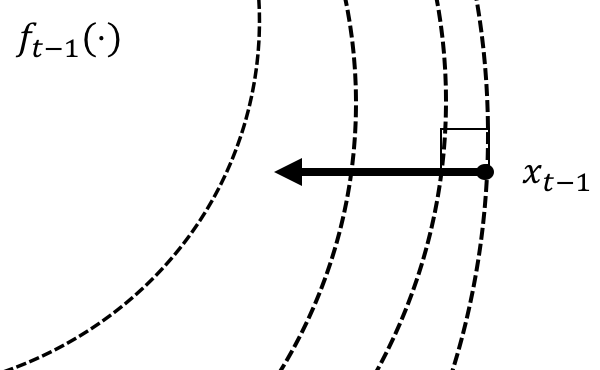
\includegraphics[width=0.23\linewidth]{comparison_5a}\hspace{.5in}}%
    \qquad \quad
    \subfigure[\textit{A step taken by \ourack. Contour lines represent the sub-level sets of $f_{t}$.}]{\label{fig: ouralg_step}%
      \hspace{.5in}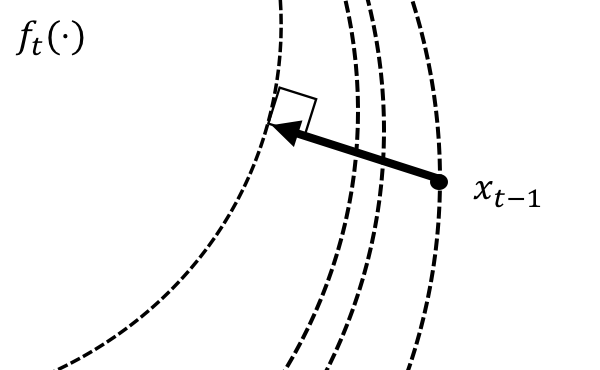
\includegraphics[width=0.23\linewidth]{comparison_5b}\hspace{.5in}}
 \vspace{-.2in}
 }
 \vspace{-.15in}
\end{figure}

For more general switching costs a similar geometric intuition can be obtained using a mirror map $\Phi$ with respect to the norm $\| \cdot \|$.  Here, $x_t$ is the solution of the following optimization in dual space where, given a convex function $\Phi$, $D_\Phi(x, y)$ is the Bregman divergence between $x$ and $y$, i.e., $D_\Phi(x, y) = \Phi(x) - \Phi(y) - \nabla \Phi(y)^T(x-y)$: 
\begin{align*}
\text{minimize}  \quad D_{\Phi}(x, x_{t-1}) \qquad
\text{subject to} \quad f_t(x) \le l.
\end{align*}
As before, let $\eta_t$ be the optimal dual variable for the inequality constraint. The first order optimality condition implies that $x_t$ must satisfy 
\begin{equation}
\nabla \Phi(x_t) = \nabla \Phi(x_{t-1}) - \eta_t \nabla f_t (x_t).
\label{eqn: mirror-descent-step}
\end{equation}
The form of \eqref{eqn: mirror-descent-step} is similar to a ``one step ahead'' version of OMD with time varying $\eta_t$, i.e., the update direction in the dual space is in the gradient $\nabla f_t(x_t)$ instead of the gradient $\nabla f_{t-1}(x_{t-1})$. The implicit form of the update has been widely used in online learning, e.g., \cite{kivinen1997exponentiated, kulis2010implicit}.

Figure \ref{fig: comparison} illustrates the difference between \ourack\ and OMD when $\Phi(x) = \frac{1}{2}\norm{x}^2_2$: \ourack\ is normal to the destination whereas OMD is normal to the starting point. Intuitively, this is why the guarantees we obtain for \ourack\ are stronger than what previous descent-based approaches have obtained in this setting -- it is better to move in the direction determined by the level set where you land, than the direction determined by the level set where you start. 

\subsection{A Meta Algorithm}
\label{sec:alg-description}

The previous section gives intuition about one key aspect of the algorithm, the projection onto a level-set.  But, in the discussion above we assume we are projecting onto a specific $l$-sublevel set. The core of \ourack\ is that this sublevel set is determined endogenously in order to ``balance'' the switching and hitting costs, as opposed to a fixed exogenous schedule of step-sizes like is typical in many online descent algorithms. Informally, the operation of \ourack\ is summarized in the \emph{meta algorithm} in Algorithm \ref{alg: online-projection}, which uses the operator $\Pi^\Phi_K(x) : \mathbb{R}^n \rightarrow K$ to denote the Bregman projection of $x$ onto a convex set $K$, i.e., $\Pi^\Phi_K(x) = \argmin_{y \in K} D_\Phi(y, x)$, where $\Phi$ is $m$-strongly convex and $M$-Lipschitz smooth in $\norm{\cdot}$, i.e., $ \frac{m}{2} \norm{x-y}^2 \le D_\Phi(x,y) \le \frac{M}{2} \norm{x-y}^2.$



We term Algorithm \ref{alg: online-projection} a meta algorithm because the general framework given in Algorithm \ref{alg: online-projection} can be instantiated with different forms of ``balance'' in order to perform well for different metrics.  More specifically, the notion of ``balance'' in the Step \ref{alg:meta-balance} that is appropriate varies depending on whether the goal is to perform well for competitive ratio or for regret.  

Our results in this paper highlight two different approaches for defining \emph{balance} in \ourack\ based on either balancing the switching cost with the hitting cost in either the primal or dual space.  We  balance costs in the primal space to yield a constant, dimension-free competitive algorithm for locally polyhedral cost functions (Section \ref{sec: alg-cr}), and balance in the dual space to yield a no-regret algorithm (Section \ref{sec: alg-regret}). We summarize these two approaches in the following and then give more complete descriptions in the corresponding technical sections.  

%\adam{Need to reincorporate the following: Let $x(l) = \Pi^\Phi_{K_l}(x_{t-1})$.  }

\begin{algorithm}[t]
	\begin{algorithmic}[1]
			\REQUIRE Starting point $x_0$, mirror map $\Phi$.
			\FOR{$t=1, \ldots, T$}
			\STATE Choose a sublevel set $K_l = \{ x \mid f_t(x) \le l\}$ to ``balance'' the switching and hitting costs.  \label{alg:meta-balance}
			  \STATE Set $x_t = \Pi^{\Phi}_{K_l}(x_{t-1})$.
              \label{alg: gradient-step}
			\ENDFOR
	\end{algorithmic}
\caption{\ouralg\ (\ourack), Meta Algorithm}
\label{alg: online-projection}
\end{algorithm}

\begin{itemize}
\item{\textbf{Primal \ouralg}}.  The algorithm we consider in Section \ref{sec: alg-cr} instantiates Algorithm \ref{alg: online-projection} by choosing $l$ such that $x(l) = \Pi^\Phi_{K_l}(x_{t-1})$ achieves balance between the switching cost with the hitting cost in the \emph{primal} space. Specifically, for some fixed $\beta>0$, choose $l$ such that either $x(l) = \argmin_x f_t(x)$ and $\norm{x(l) - x_{t-1}} < \beta l $, or the following is satisfied:
\begin{equation}
\norm{x(l) - x_{t-1}} = \beta l
\label{eqn: primal-balance}
\end{equation}

\item{\textbf{Dual \ouralg}}. The algorithm we consider in Section \ref{sec: alg-regret} instantiates Algorithm \ref{alg: online-projection} by balancing the switching cost with the size of the gradient in the \emph{dual} space.  Specifically, for some fixed $\eta$, we choose $l$ such that 
\begin{equation}
\norm{\nabla \Phi(x(l)) - \nabla \Phi(x_{t-1})}_* = \eta \norm{\nabla f_t(x(l))}_*,
\label{eqn: dual-balance}
\end{equation}
\end{itemize}

The final piece of the algorithm is computational.  Note that the algorithm is \emph{memoryless}, i.e., it does not use any information about previous cost functions.  Thus, the only question about efficiency is whether the appropriate $l$ can be found efficiently.  The following lemmas verify that, indeed, it is possible to compute $l$, and thus implement \ourack, efficiently.  

\begin{lemma}
		The function $g(l) = \norm{x(l) - x_{t-1}}$ is continuous in $l$. 
		\label{lem: continuity-distance}
\end{lemma}

\begin{lemma}
Consider $\Phi$ and $f_t$ that are continuously differentiable on $\mathcal{X}$. The function \\ $h(l) = \frac{\norm{\nabla \Phi(x_{t-1}) - \nabla \Phi(x(l)) }_*}{\norm{\nabla{f_t(x(l))}}_*}$ is continuous in $l$. 
\label{lem: continuity-ratio}
\end{lemma}

The continuity of $g(l)$ and $h(l)$ in $l$ is enough to guarantee efficient implementation of Primal and Dual \ourack\ because it shows that an $l$ satisfying the balance conditions in the algorithms exists and, further, can be found to arbitrary precision via bisection.  Proofs are included in the appendix.

\subsection{Examples}
\label{sec:alg-examples}

An important part of the design of an \ourack\ algorithm is the choice of the mirror map.  
%Recall that \ourack\ needs to choose a mirror map that is both strongly convex and Lipschitz smooth for the norm defined by the switching cost. Clearly, 
Different choices of a mirror map $\Phi$ can lead to very different behavior by the resulting algorithms. To highlight this, and give intuition for the impact of the choice, we describe three examples of mirror maps below.  These examples focus on mirror maps that are commonly used for OMD, and they highlight interesting connections between the \ourack\ framework and classical online optimization algorithms like OGD \citep{zinkevich2003} and Multiplicative Weights \citep{arora2012}.

\paragraph{Euclidean norm squared:} Consider $\Phi(x) = \frac{1}{2}\norm{x}_2^2$, which is both 1-strongly convex and 1-Lipschitz smooth for the $\ell_2$ norm. Note that $\nabla \Phi(x) = x$.  Then, the first order condition \eqref{eqn: mirror-descent-step} is 
\begin{equation}
x_t = x_{t-1} - \eta_t \nabla f_t(x_t).
\label{eqn: one-step-ahead-GD}
\end{equation}
Interestingly, this can be interpreted as a ``one-step ahead'' OGD (illustrated in Figure \ref{fig: comparison}).  However, note that this equation should not be interpreted as an update rule since $x_t$ appears on both side of the equation.  In fact, this contrast highlights an important difference between OGD and \ourack.

\paragraph{Mahalanobis distance square:} Consider $\Phi(x) = \frac{1}{2} \norm{x}_Q^2$ for positive definite definite $Q$, which is 1-strongly convex and 1-Lipschitz smooth in the Mahalanobis distance $\norm{\cdot}_Q$.  Note that $\nabla \Phi(x) = Qx$.  Then, the first order condition \eqref{eqn: mirror-descent-step} is 
\begin{equation}
x_t = x_{t-1} - \eta_t Q^{-1} \nabla f_t(x_t).
\label{eqn: one-step-ahead-weighted-GD}
\end{equation}
This is analogous to a ``one step ahead" OGD where the underlying metric is a weighted $\ell_2$ metric.

\paragraph{Negative entropy:} If the feasible set is the $\delta$-interior of the simplex $\mathcal{X} = P_\delta = \{ x \mid \sum_{i=1}^n x_i = 1, x_i \ge \delta\}$, and the norm is the $\ell_1$ norm $\norm{\cdot}$, the mirror map defined by the negative entropy $\Phi(x) = \sum_{i=1}^n x_i \log x_i$ is $\frac{1}{2\ln 2}$-strongly convex (by Pinsker's inequality) and $ \frac{1}{\delta \ln 2}$-Lipschitz smooth (by reverse Pinsker's inequality \citep{sason2015}). In this case, $\nabla \Phi(x) = \log x + 1_d$, where $1_d$ represents the all 1s vector in $\mathbb{R}^d$. Then, the first order condition is 
\begin{equation}
x_t =  x_{t-1}\exp(-\eta_t \nabla f_t(x_t)).
\label{eqn: one-step-ahead-multiplicative-weight}
\end{equation}
This can be viewed as a ``one-step ahead'' version of the multiplicative weights update. Again, this equation should not be interpreted as an update rule since $x_t$ appears on both side of the equation.







\section{A Competitive Algorithm}
\label{sec: alg-cr}
%!TEX root = LookingGlass.tex

In this section, we use the \ourack\ framework to give the first algorithm with a dimension-free, constant competitive ratio for online convex optimization with switching costs in general Euclidean spaces, under mild assumptions on the structure of the cost functions.  Recall that, for the most general case, where no constraints other than convexity are applied to the cost functions, Proposition \ref{prop: lowerbound} shows that the competitive ratio of any online algorithm must be $\Omega(\sqrt{d})$ for $\ell_2$ switching costs, i.e., must grow with the dimension $d$ of the decision space. Our goal in this section is to understand when a dimension-free, constant competitive ratio can be obtained.  Thus, we are naturally led to restrict the type of cost functions we consider. 
 
Our main result in this section is a new online algorithm whose competitive ratio is constant with respect to dimension when the cost functions are \emph{locally polyhedral}, a class that includes the form of cost functions used in many applications of online convex optimization, e.g, tracking problems and penalized estimation problems. Roughly speaking, locally polyhedral functions are those that grow at least linearly as one moves away from the minimizer, at least in a small neighborhood. 

\begin{definition}
A function $f_t$ with minimizer $v_t$ is \textbf{\textit{locally $\alpha$-polyhedral}} with respect to the norm $\| \cdot \|$ if there exists some $\alpha, \epsilon > 0$, such that for all $x \in \mathcal{X}$ such that $\norm{x - v_t} \le \epsilon$, $f_t(x) - f_t(v_t)\ge  \alpha \norm{x - v_t}$.
\label{locallypolyhedraldef}
\end{definition}

Note that all strictly convex functions $f_t$ which are locally $\alpha$-polyhedral automatically satisfy $f_t(x) - f_t(v_t) \ge \alpha \norm{x - v_t}$ for all $x$, not just those $x$ which are $\epsilon$ close to the minimizer $v_t$. In this setting, local polyhedrality  is analogous to strong convexity; instead of requiring that the cost functions grow at least quadratically as one moves away from the minimizer, the definition requires that cost functions grow at least linearly. The following examples illustrate the breadth of this class of functions. One important class of examples are functions of the form $\|x - v_t \|_a$ where $\| \cdot \|_a$ is an arbitrary norm; it follows from the equivalence of norms that such functions are locally polyhedral with respect to any norm. Intuitively, such functions represent ``tracking'' problems, where we seek to get close to the point $v_t$. Another important example  is the class $f(x_t) = g(x_t) + h(x_t)$ where $g$ is locally polyhedral and $h$ is an arbitrary non-negative convex function whose minimizer coincides with that of $g$; since $f(x_t) - f(v_t) \geq g(x_t) - g(v_t)$, $f$ is also locally polyhedral. This lets us handle interesting functions such as $f(x_t) = \|x_t\|_1 + x_t' Q x_t$ with $Q$ psd, or even $f(X_t) = 2\|X_t\|_{\infty}  -\log{\det{\left( I + X_t \right)}}$ where the decision variable $X_t$ is a PSD matrix. Note that locally polyhedral function have previously been applied in the networking community, e.g., by \cite{huang2011} to study delay-throughput trade-offs for stochastic network optimization and by \cite{lin2012} to design online algorithm for geographical load balancing in data centers.   
 
Let us now informally describe how the \ouralg\ framework described in Section \ref{sec: alg-meta} can be instantiated to give a competitive online algorithm for locally polyhedral cost functions.  \ouralg\ is, in some sense, \textit{lazy}: instead of moving directly towards the minimizer $v_t$, it moves to the closest point which results in a suitably large decrease in the hitting cost. This can be interpreted as projecting onto a sublevel set of the current cost function. The trick is to make sure that not too much switching cost is incurred in the process. This is accomplished by carefully picking the sublevel set so that the hitting costs and switching costs are balanced. A formal description is given Algorithm \ref{alg: online-projection-CR}. By Lemma \ref{lem: continuity-distance}, step \ref{projection-step-cr} can be computed efficiently via bisection on $l$. Note that the memoryless algorithm proposed in \cite{bansal2015} can be seen as a special case of Algorithm \ref{alg: online-projection-CR} when the decision variables are scalar. %Additionally note that Algorithm \ref{alg: online-projection-CR} can be implemented efficiently using the bisection method presented in Section \ref{sec: alg-meta}.


\begin{algorithm}[t]
	\begin{algorithmic}[1]
% 		\REQUIRE Initial state $x_0$, mirror map $\Phi$, balance parameter $\beta \in (\frac{2\sqrt{\kappa}-1}{\alpha}, 1)$.
			\FOR{$t=1, \ldots, T$}
                  \STATE Observe cost function $f_t$, set $v_t = \argmin_{x} f_t(x)$.
			\IF{$\norm{x_{t-1}-v_t} < \beta f_t(v_t)$}
            \STATE Set $x_t = v_t$ 
            \ELSE
			\STATE Let $x(l) = \Pi_{K_t^l}^\Phi (x_{t-1})$,
            %\argmin_{x \in K_l} D_\Phi(x, x_{t-1})$, 
            increase $l$ until $\norm{x(l) - x_{t-1}} = \beta l$. Here $K_t^l$ is the $l$-sublevel set of $f_t$, i.e., $K_t^l = \{ x \mid f_t(x) \le l\}$. 
			\label{projection-step-cr}
            \STATE $x_t = x(l)$.
            \ENDIF
			\ENDFOR
	\end{algorithmic}
\caption{(Primal) \ouralg}
\label{alg: online-projection-CR}
\end{algorithm}



%\adam{rewrite the discussion of the algorithm so that it makes sense indpendently of the pseudocade.  Basically, write it like "To apply the meta-algorithm in this context we ... This is summarized in Algorithm 2} The key step in Algorithm \ref{alg: online-projection-CR} is step \ref{projection-step-cr}, where we carefully pick a sublevel set so as to precisely balance the hit cost $f_t(x_t)$ and the movement cost $\norm{x_t - x_{t-1}}$; the parameter $\beta$ trades off between the two. 


 

The main result of this section is a characterization of the competitive ratio of Algorithm \ref{alg: online-projection-CR}.

% The key idea of choosing $K_l$ in step \ref{alg: gradient-step} of Algorithm \ref{alg: online-projection} is to strike balance between movement cost and hit cost (or size of the gradient). In the following lemma we show that there exist an $l$ that achieve such balance, moreover, we find such $l$ efficiently via bisection. The proof is included in the Appendix. 
% %Note that the hit cost $f_t(x_t) = l$, and the movement cost $\norm{x_t - x_{t-1}} = \norm{x_{t-1}, K_l}$ where we define the distance from a point to a convex set $d(u, K) = \min_{v \in K} \norm{u-v}$. 
% \begin{lemma}
% 		Let $x(l) = \argmin_{K_l} D_{\Phi}(x, x_{t-1}) $. The function $g(l) = \norm{x(l) - x_{t-1}}$ is continuous in $l$. 
% 		\label{lem: continuity-distance}
% \end{lemma}



% Given Lemma \ref{lem: continuity-distance}, let $l_0 = f_t(v_t)$, and $l_1 = f_t(x_{t-1})$,  we know that $ g(l_0) > \beta l_0 $, and $0 = g(l_1) < \beta l_1$. By intermediate value theorem, there exists $l_0 < l < l_1$ such that $ g(l) = \beta l$, i.e., $\norm{x_t - x_{t-1}} = \beta f_t(x_t)$.

% Further, by continuity of the function  $ g(l) - \beta l$, we can use bisection to find $l$ such that $g(l) = \beta l$. Computing the projection $\Pi_{K_l}(x_{t-1})$ for each individual $l$ is a convex problem, hence we can compute step \ref{projection-step-cr} in polynomial time independent of $T$.


\begin{theorem}
\label{threeCR}
For every $\alpha > 0$, there exists a choice of $\beta$ such that Algorithm \ref{alg: online-projection-CR} has competitive ratio at most $3 + O(1/\alpha)$ when run on locally $\alpha$-polyhedral cost functions with $\ell_2$ switching costs. More generally, let $\| \cdot \|$ be an arbitrary norm. There exists a choice of $\beta$ such that Algorithm \ref{alg: online-projection-CR} has competitive ratio at most $\frac{\max\{k_2, 1\}}{\min\{k_1, 1\}} \left(3 + O(1/\alpha)\right)$ when run on locally $\alpha$-polyhedral cost functions with switching cost $\| \cdot \|$. Here  $k_1$ and $k_2$ are constants such that $k_1\norm{x} \le \norm{x}_2 \le k_2\norm{x}$.  
\end{theorem}

We note that in the $\ell_2$ setting Theorem \ref{threeCR} has a form which is connected to the best known lower bound on the competitive ratio of memoryless algorithms. In particular, \cite{bansal2015} use a 1-dimensional example with locally polyhedral cost functions to prove the following bound. 

\begin{proposition} No memoryless algorithm can have a competitive ratio less than 3. 
\label{thm: lower-bound}
\end{proposition}

%\noindent Thus, for the $L_2$ setting Algorithm \ref{alg: online-projection-CR} is only $O(1/\alpha)$ from this lower bound. 

Beyond the $\ell_2$ setting, the competitive ratio in Theorem \ref{threeCR} is no longer dimension-free.  It is interesting to note that, when the switching costs are $\ell_1$ or $\ell_{\infty}$ and $\alpha$ is fixed, \ouralg\ has a competitive ratio that is $O(\sqrt{d})$. In particular, we showed in Section \ref{sec: model} that for general cost functions, there is a $\Omega(d)$ lower bound on the competitive ratio for SOCO with $\ell_{\infty}$ switching costs; hence our $O(\sqrt{d})$ result highlights that local polyhedrality is useful beyond the $\ell_2$ case.

%, matching the lower bound in \cite{Friedman1993} and \cite{antoniadis2016}.  \niangjun{Not quite true. That bound is only valid for $l_2$ case. If you go through their example, they showed a competitive ratio of $d / \norm{1_d}$ where $1_d$ is the all 1 vector. So CR is $\sqrt{d}$ if the norm is $l_2$, $d$ if norm is $l_\infty$, and 1 if norm is in $l_1$.}

While Theorem \ref{threeCR} suggests that \ouralg\ has a constant (dimension-free) competitive ratio only in the $\ell_2$ setting, a more detailed analysis shows that it can be constant-competitive outside of the $\ell_2$ setting as well, though for a more restrictive class of locally polyhedral functions.  This is summarized in the the following theorem.

\begin{theorem}\label{generalconstant}
Let $\| \cdot \|$ be any norm such that the corresponding mirror map $\Phi$ has Bregman divergence $D_{\Phi}$ satisfying $\frac{m}{2}\norm{x-y}^2 \le D_{\Phi}(x,y) \le \frac{M}{2}\norm{x-y}^2$  
for all $x, y \in \mathbb{R}^d$ and some positive constants $m$ and $M$. Let $\kappa = M/m$. For every $\alpha > 2\sqrt{\kappa - 1}$, there exists a choice of $\beta$ so that Algorithm \ref{alg: online-projection-CR} has competitive ratio at most $3 + O(1/\alpha)$ when run on locally $\alpha$-polyhedral cost functions with switching costs given by $\| \cdot \|$.
\end{theorem}

This theorem highlights that for any given locally polyhedral cost functions, the task of finding a constant-competitive algorithm can be reduced to finding an appropriate $\Phi$.  In particular, given a class of polyhedral cost functions with $\alpha >0$ and norm $\norm{\cdot}$, the problem of finding a dimension-free competitive algorithm can be reduced to finding a convex function $\Phi$ that satisfies the differential inequality $\frac{1}{2}\norm{x-y}^2\le \Phi(x) - \Phi(y) - \langle \nabla \Phi(y), x - y\rangle \le \frac{\alpha^2+4}{8}\norm{x-y}^2$ for all $x,y \in \mathcal{X}$.



%Now, let us return to the proof of Theorem \ref{threeCR}. Before giving the formal argument, 
We present an intuitive overview of our proof techniques here, and defer the details to the appendix. We use a potential function argument to bound the difference in costs paid by our algorithm and the offline optimal.  Our potential function tracks the distance between the points $x_t$ picked by our algorithm and the points $x_t^*$ picked by the offline optimal. 
%Using a simple triangle inequality argument, we observe we may assume that in each round the offline algorithm has already moved; this simplifies the analysis since we do not need to consider the offline movement cost.
There are two cases to consider. Either the online point or the offline point has smaller hit cost. The first case is easy to deal with, since our algorithm is designed so that the movement cost is at most a constant $\beta$ times the hit cost; hence if our online hit cost is less than the offline algorithm's hit cost, our total per-step cost will at most be a constant times what the offline paid. The second case is more difficult. The key step is Lemma  \ref{lem: potential-change}, where we show that the potential must have decreased if the offline has smaller hit cost. We use this fact to argue that the total per-step cost we charge \ouralg, namely the sum of the hit cost, movement cost, and change in potential, must be non-positive. 

% In this section we discuss performance guarantee for functions that are polyhedral, i.e., there exists $\alpha >0$ such that $f_t(x) \ge \alpha \norm{x - v_t}$ for all $t$. Note that \textit{locally polyhedral} function\footnote{there exist $\epsilon, L>0$, such that for all $x \in \mathcal{X}$ with $\norm{x - v_t} \le \epsilon$, $f_t(x) \ge f_t(v_t) + L\norm{x - v_t}$.} used in \cite{huang2011} to show $(\log^2(V), 1/V)$ trade-off in queue size utility trade-off in stochastic network optimization problem are polyhedral functions. The polyhedral property also holds for convex functions that are increasing, $\mathcal{X} \subset \mathbb{R}^n_+$, and $f(x) \ge c x$ as used in \cite{lin2012}. 

% \begin{theorem}
% Let $\Phi$ be $m$-strongly convex and $M$-smooth in $\norm{\cdot}$ and let $\kappa = M / m$. For polyhedral function $f_t$ where there exists $\alpha>2\sqrt{\kappa -1}$, such that $f_t(x_t) \ge \alpha \norm{x_t - v_t}, \forall t$.  Algorithm \ref{alg: online-projection} with $\beta \in \left(\frac{2\sqrt{\kappa-1}}{\alpha}, 1\right)$ is $C$-competitive for $C = \max \left\{ \frac{1+\beta}{1-\beta}, \frac{1+\beta}{\beta} \frac{1}{\gamma}\right\}$, where $\gamma = \frac{1}{\sqrt{\kappa}}\sqrt{1 + \left( \frac{2}{\alpha\beta}\right)^2} - \frac{2}{\alpha\beta}$.
% %\niangjun{ substituting $\gamma$ gives \[ C = \max \left \{ \frac{1+\beta}{1-\beta} , \frac{1+\beta}{\beta} \left( \frac{ \sqrt{\kappa}\left( \sqrt{ 1 + \left(\frac{2}{\alpha\beta}\right)^2 } + \frac{2}{\alpha\beta}\sqrt{\kappa} \right) }{ 1 + \left( \frac{2}{\alpha\beta}\right) - \frac{2}{\alpha\beta} \sqrt{\kappa}} \right)\right\}. 
% %\]}
% \label{thm: competitive-ratio}
% \end{theorem}

% Theorem \ref{thm: competitive-ratio} shows that, whenever $\alpha > 2\sqrt{\kappa-1}$, for any $\beta \in (0, 1)$, Algorithm \ref{alg: online-projection-CR} is constant competitive, where the constant is \textit{dimension-free}. Furthermore, as $C$ is positively correlated to $\kappa$, we should choose mirror map $\Phi$ for $\norm{\cdot}$ such that $\kappa$ is small. For example, when the switching cost is measured in $2$-norm, we should use $\Phi(x) = \frac{1}{2}\norm{x}^2$ with $\kappa = 1$. 

% In addition, if we know the value of $\alpha$ apriori, we can choose $\beta$ to optimize the performance guarantee $C$ in the following manner: 

% Note that $g(\beta) = \frac{1+\beta}{1-\beta}$ is an increasing function in $\beta$, and tends to $+\infty$ as $\beta \rightarrow 1$, and $h(\beta) =  \frac{1+\beta}{\beta} \frac{1}{\gamma} $ is a decreasing function in $\beta$, and tends to $+\infty$ when $\beta \rightarrow \frac{2\sqrt{\kappa-1}}{\alpha}$, hence the value of $C = \max\{ g(\beta), h(\beta) \}$ is minimized when $\beta$ takes value such that $g(\beta) = h(\beta),$ formally stated in the following Corollary: 
% \begin{corollary}
% When $\kappa = 1$, Algorithm \ref{alg: online-projection-CR} is $(3+8/\alpha)$-competitive where $\beta = \frac{1}{2} + \frac{1}{\alpha+2},$ when $\kappa > 1$, 
% Algorithm \ref{alg: online-projection-CR} is $C$-competitive for 
% \[
% C = \frac{2 \alpha \sqrt{(\alpha^2 + 4\alpha  + 8) \kappa - 4} + \alpha^2 + 4 \alpha \kappa + 4 \kappa - 4}{\alpha^2 - 4 \kappa + 4} = 3 + O\left(\frac{1}{\alpha}\right),
% \]
% where
% \[ \beta =  \frac{(\alpha+2)\kappa - \sqrt{ (\alpha^2+4\alpha+8)\kappa-4  } }{\alpha(\kappa-1)}. 
% \]
% \label{cor: online-projection-CR}
% \end{corollary}
% \todo{1. provide some intuition about corollary 6; 2. discuss about different $\kappa$ in different norms}


%We can see that Algorithm \ref{alg: online-projection-CR} performs better for when $\alpha$ is large. This is not surprising since Algorithm \ref{alg: online-projection} in general is only acting on the current information about $f_t$, $\alpha$ can be roughly seen as the amount of information presented to the online algorithm, and larger $\alpha$ implies bigger gains in moving in the negative gradient direction.  

The proof of Theorem \ref{generalconstant} parallels that of Theorem \ref{threeCR}. The key difference is the use of a more general form of Lemma \ref{lem: potential-change}, which uses Bregman projection to show that the potential decreases. The Bregman divergence is with respect to the mirror map induced by $\| \cdot \|$. %The rest of the proof is unchanged. The general form of Lemma \ref{lem: potential-change} that is used is stated and proven in the appendix.












% In this Section, we discuss the design and analysis of high dimensional online algorithm with constant competitive ratio. Define distance from a point $u$ to a convex set $K$ to be 
% $d(u, K) = \min_{v \in K} \norm{u - v}$, and let $\beta \in (0, 1)$. The proofs of the theoretical results can be found in the Appendix.
   
% \begin{algorithm}
% 	\begin{algorithmic}[1]
% 			\FOR{$t=1, \ldots, T$}
% 			\STATE If $\norm{x_{t-1}-v_t} \le \beta f_t(v_t)$, then set $x_t = v_t$.
% 			\STATE Otherwise, increase $l$ from $l=f_t(v_t)$ until $d(x_{t-1}, K_l) = \beta l$, where $K_l$ is the $l$-sublevel set of $f_t$, i.e., $K_l = \{ x | f_t(x) \le l\}$. 
% 			\label{projection-step-cr}
% 			 \STATE $x_t = \Pi_{K_l}(x_{t-1})$.
% 			\ENDFOR
% 	\end{algorithmic}
% \caption{Online projection for constant competitive ratio}
% \label{alg: online-projection-CR}
% \end{algorithm}

% The key step in Algorithm \ref{alg: online-projection-CR} is step \ref{projection-step-cr}, which is to find a suitable sublevel set, such that the hit cost $f_t(x_t)$ and the movement cost $\norm{x_t - x_{t-1}}$ is balanced, and the parameter $\beta$ control such balance.   
% %The immediate questions for step \ref{projection-step-cr} are 
% %\begin{enumerate}
% %	\item Is it well defined?
% %	\item If so, what's the computational complexity of computing it?
% %\end{enumerate} 
% As shown in Section \ref{sec: balance-movement-hit}, step \ref{projection-step-cr} can be computed efficiently. 
% %The immediate questions are whether Step \ref{projection-step-cr} is well-defined and computationally efficient, we show that this is indeed the case by the following Lemma: 



% Note that Algorithm \ref{alg: online-projection-CR} can be viewed as a generalization of the memoryless algorithm proposed in \cite{bansal2015} when the decision variables are scalar. 




% \subsection{Polyhedral Functions}
% In this section we discuss performance guarantee for functions that are polyhedral, i.e., there exists $\alpha >0$ such that $f_t(x) \ge \alpha \norm{x - v_t}$ for all $t$. Note that \textit{locally polyhedral} function\footnote{there exist $\epsilon, L>0$, such that for all $x \in \mathcal{X}$ with $\norm{x - v_t} \le \epsilon$, $f_t(x) \ge f_t(v_t) + L\norm{x - v_t}$.} used in \cite{huang2011} to show $(\log^2(V), 1/V)$ trade-off in queue size utility trade-off in stochastic network optimization problem are polyhedral functions. The polyhedral property also holds for convex functions that are increasing, $\mathcal{X} \subset \mathbb{R}^n_+$, and $f(x) \ge c x$ as used in \cite{lin2012}. 

% \begin{theorem}
% For polyhedral function $f_t$, i.e., there exists $\alpha>0$, such that $f_t(x_t) \ge \alpha \norm{x_t - v_t}, \forall t$.  Algorithm \ref{alg: online-projection} is $C$-competitive for $C = \max \left \{ \frac{1+\beta}{1-\beta} , \frac{1+\beta}{\beta} \left( \sqrt{\left(\frac{2}{\alpha\beta}\right)^2 + 1}  + \frac{2}{\alpha\beta} \right)\right\}$ for $\beta \in (0, 1)$. 
% \label{thm: competitive-ratio}
% \end{theorem}

% Theorem \ref{thm: competitive-ratio} shows that, whenever $\alpha > 0$, for any $\beta \in (0, 1)$, Algorithm \ref{alg: online-projection-CR} is constant competitive, where the constant is \textit{dimension-free}. In addition, if we know the value of $\alpha$ apriori, we can choose $\beta$ to optimize the performance guarantee $C$ in the following manner: 

% Note that $g(\beta) = \frac{1+\beta}{1-\beta}$ is an increasing function in $\beta$, and tends to $+\infty$ as $\beta \rightarrow 1$, and $h(\beta) =  \frac{1+\beta}{\beta} \left( \sqrt{\left(\frac{2}{\alpha\beta}\right)^2 + 1}  + \frac{2}{\alpha\beta} \right) $ is a decreasing function in $\beta$, and tends to $+\infty$ when $\beta \rightarrow 0$, hence the value of $C = \max\{ g(\beta), h(\beta) \}$ is minimized when $\beta$ takes value such that $g(\beta) = h(\beta),$ formally stated in the following Corollary: 
% \begin{corollary}
% Algorithm \ref{alg: online-projection-CR} is $3+8/\alpha$-competitive when $\beta = \frac{1}{2} + \frac{1}{\alpha+2}$.
% \label{cor: online-projection-CR}
% \end{corollary}
% We can see that Algorithm \ref{alg: online-projection-CR} performs better for when $\alpha$ is large. This is not surprising since Algorithm \ref{alg: online-projection} in general is only acting on the current information about $f_t$, $\alpha$ can be roughly seen as the amount of information presented to the online algorithm, and larger $\alpha$ implies bigger gains in moving in the negative gradient direction.  
% \begin{proof}[Theorem \ref{thm: competitive-ratio}]
% Let $H_t = f_t(x_t), M_t=\norm{x_t - x_{t-1}}$. Using potential function $\phi_t = C \norm{x_t - x_{t-1}}$, where $\phi_0 = 0$. To show Algorithm \ref{alg: online-projection-CR} is $C$-competitive, we just need to show that for all $t$,
% \begin{equation}
%  	H_t + M_t + \phi_t - \phi_{t-1} \le C(H_t^* + M_t^*),
%     \label{eqn: potential-ineq}
% \end{equation}
% then summing up the inequality over $t$ implies the result.

% Firstly, since 
% \begin{align}
% 	\phi_t - \phi_{t-1} &= C (\norm{x_t - x_t^*} - \norm{x_{t-1} - x_{t-1}^*}) \notag \\
% 	&= C ( \norm{x_t - x_t^*} - \norm{x_t^* - x_{t-1}} + \norm{x_t^* - x_{t-1}} -  \norm{x_{t-1} - x_{t-1}^*}) \notag \\
% 	&\le C  (\norm{x_t - x_t^*} - \norm{x_t^* - x_{t-1}}) + C M_t^*
%     \label{eqn: potential-change}
% \end{align}
% Combining \eqref{eqn: potential-change} and \eqref{eqn: potential-ineq}, we can show Algorithm \ref{alg: online-projection-CR} is $C$-competitive by show that 
% \[
% 	H_t + M_t + C (\norm{x_t - x_t^*} - \norm{x_t^* - x_{t-1}}) \le C H_t^*, \tag{$\dagger$}
% \]
% We divide our analysis to the following two cases:

% \begin{enumerate}
% 	\item $H_t \le H_t^*$: in this case, $M_t \le \beta H_t$, by the triangle inequality,
% 	\begin{align*} 
% 		&H_t + M_t + C (\norm{x_t - x_t^*} - \norm{x_t^* - x_{t-1}}) \\
% 		\le & H_t + (1+C) M_t \le (1 + \beta(1+C))H_t \le CH_t^*,
% 	\end{align*}
% 	the last inequality sign holds when $C \ge\frac{1+\beta}{1 - \beta}$. 
% 	\item $H_t > H_t^*$: in this case, $M_t = \beta H_t$,  we use the following Lemma:  
% \begin{lemma}
% 	For Algorithm \ref{alg: online-projection-CR}, when $H_t > H_t^*$ and $f_t(x) \ge \alpha\norm{x - v_t}$, we have 
% 	\[ \norm{x_t - x_t^*} - \norm{x_t^* - x_{t-1} } \le -\gamma \norm{x_t - x_{t-1}}, \]
% 	where $\gamma = \sqrt{(\frac{2}{\alpha\beta})^2+1} - \frac{2}{\alpha\beta}$.
% 	\label{lem: potential-change}
% \end{lemma}
%  With Lemma \ref{lem: potential-change}, we have 
% \begin{align*} 
% 	&H_t + M_t + C (\norm{x_t - x_t^*} - \norm{x_t^* - x_{t-1}}) \\
% 	\le & H_t + M_t - C (\gamma M_t) = (1 + \beta(1 - C\gamma)) H_t
% \end{align*}
% To show $(\dagger)$, we just need $ 1 + \beta \left (1 - C \gamma \right) \le 0, $
% which is equivalent to $C \ge \frac{1+\beta}{\beta} \cdot \frac{1}{\gamma}$. Substitute $\gamma = \sqrt{(\frac{2}{\alpha\beta})^2+1} - \frac{2}{\alpha\beta}$ from Lemma \ref{lem: potential-change}, $(\dagger)$ holds in this case if 
% \[
% C \ge \frac{1+\beta}{\beta} \left(\sqrt{\left(\frac{2}{\alpha\beta}\right)^2+1}+\frac{2}{\alpha\beta}\right),
% \]
% \end{enumerate}
% Combining case 1 and 2, we conclude that Algorithm \ref{alg: online-projection-CR} is $C$-competitive for 
% \[C = \max \left \{ \frac{1+\beta}{1-\beta} , \frac{1+\beta}{\beta} \left( \sqrt{\left(\frac{2}{\alpha\beta}\right)^2 + 1}  + \frac{2}{\alpha\beta} \right)\right\},\] 
% which completes the proof.
% \end{proof}


% \subsection{Generalizing to arbitrary norms}
% \gautam{It's definitely important that we mention this and give lots of example. My suspicion is that this is a bit too trivial to merit its own section with a full proof; everyone at COLT will understand this immediately}
% We can generalize the results in Theorem \ref{thm: competitive-ratio} and Corollary \ref{cor: online-projection-CR} to arbitrary norms for Algorithm \ref{alg: online-projection-CR}. Note that in the finite dimensional space, all norms are equivalent up to a constant, i.e., for all norms $\norm{\cdot}_a$, there exists $k_1, k_2 >0$, such that 
% $ k_1\norm{x}_a \le \norm{x} \le k_2\norm{x}_a.$
% \niangjun{note that this requires running Algorithm 2 with the Euclidean norm instead of the norm defined by the switching cost}
% \begin{corollary}
% For any norm $\norm{\cdot}_a$, such that $k_1 \norm{x}_a \le \norm{x} \le k_2 \norm{x}_a$ for all $x \in \mathbb{R}^n$, then if Algorithm \ref{alg: online-projection-CR} is $C$-competitive in Euclidean norm, then it is $\left(C \frac{\max\{k_2, 1\}}{\min\{k_1, 1\}} \right)$-competitive in $\norm{\cdot}_a$.   
% \label{cor: general-norms}
% \end{corollary}
% \begin{proof}[Corollary \ref{cor: general-norms}]
% Since $f_t(x) \ge 0$ for all $x$, and norms are always non-negative, we have 
% \begin{align}
% \label{eqn: norm1}
% \sumt f_t(x_t) + \norm{x_t - x_{t-1}} &\ge \min\{1, k_1\} \left(\sumt f_t(x_t) + \norm{x_t - x_{t-1}}_a\right) \\
% \label{eqn: norm2}
% \sumt f_t(x_t^*) + \norm{x_t^* - x_{t-1}^*} &\le \max\{1, k_2\} \left(\sumt f_t(x_t^*) + \norm{x_t^* - x_{t-1}^*}_a\right) 
% \end{align}
% Combining \eqref{eqn: norm1} and \eqref{eqn: norm2} with $ \sumt f_t(x_t) + \norm{x_t - x_{t-1}} \le C \left(\sumt f_t(x_t^*) + \norm{x_t^* - x_{t-1}^*}\right)$ finishes the proof. 
% \end{proof}



% We show in this section that we can balance between the movement cost and the hit cost by choosing the sublevel set $K_l$ in an efficient manner. %In Section \ref{sec: alg-cr} we show that balancing the movement cost and the hit cost lead to a constant competitive algorithm that is dimension free.


\section{A No-regret Algorithm} 
\label{sec: alg-regret}

\begin{algorithm} [t]
\begin{algorithmic}[1]
\FOR{$t=1, \ldots, T$}
			\STATE Define $x(l) = \Pi^\Phi_{K_l}(x_{t-1})$, increase $l$ from $l=f_t(v_t)$, until $\norm{\nabla \Phi(x(l)) - \nabla \Phi(x_{t-1})}_* = \eta \norm{\nabla f_t (x(l))}_*$. 
			\label{projection-step-regret}
			\STATE $x_t =  x(l)$.
			\ENDFOR
\end{algorithmic}
\caption{(Dual) \ouralg}
\label{alg: online-projection-regret}
\end{algorithm}

%We now move from competitive ratio to regret, specifically dynamic regret.  
While the online algorithms community typically focuses on competitive ratio, regret is typically the focus of the online learning community. The difference in performance metrics leads to differences in the settings considered.  In the previous section, we studied locally polyhedral cost functions, while here we focus on cost functions that are continuously differentiable and have a minimizer $v_t$ in the interior of the feasible set $\mathcal{X}$.\footnote{Any convex function can be approximated by a convex functions with these properties, e.g., see \cite{nesterov2005}.% and \cite{wright1999}.
}  

Interestingly, it is has been shown that the change in metric from competitive ratio to regret has a fundamental impact on the type of algorithms that perform well. Concretely, it has been shown that no single algorithm can perform well across (static) regret and competitive ratio \citep{andrew2013}.  Consequently, it is not surprising that we find a different choice of balance in \ourack\ is needed to obtain the no-regret performance guarantees.  Specifically, in contrast to the results of the previous section, which focus on a form of balance in the primal setting, in this section we focus on balance in the dual setting, where we compare costs as measured in the dual norm, $\norm{x}_* = \max_{\norm{z} \le 1} \langle z, x \rangle$. 

We show that choosing  $l$ to balance between the switching cost in the dual space and the size of the gradient leads to an online algorithm with small dynamic regret. It is worth emphasizing that, in contrast to the results of the previous section, we balance the switching cost against the marginal hitting cost $\norm{\nabla f_t(x_t)}_*$ instead of $f_t(x_t)$. A formal description of the instantiation of \ourack\ for regret is given in Algorithm \ref{alg: online-projection-regret}, which can be implemented efficiently via bisection (Lemma \ref{lem: continuity-ratio}).% implies that the right balance can be computed efficiently via bisection when implementing Step \ref{projection-step-regret}. Our main result in this section bounds the dynamic regret of Algorithm \ref{alg: online-projection-regret}. 

\begin{theorem}
Consider $\Phi$ that is an $m$-strongly convex function in $\norm{\cdot}$ with $\norm{\nabla \Phi(x)}_*$ bounded above by $G$ and $\nabla \Phi(0) = 0$. Then the $L$-constrained dynamic regret of Algorithm \ref{alg: online-projection-regret} is $\leq \frac{GL}{\eta}  + \frac{T\eta}{2m}.$
\label{thm: online-projection-regret}
\end{theorem} 

While the result above does not depend on knowing the parameters of the instance, if we know the parameters $T$, $D$ and $L$ ahead of time then we can optimize the balance parameter $\eta$ as follows.

\begin{corollary}\label{cor: online-projection-regret}
When $\eta =\sqrt{\frac{2GLm}{T}}$,  Algorithm \ref{alg: online-projection-regret} has $L$-constrained dynamic regret $\leq \sqrt{\frac{2GLT}{m}}.$ 
\end{corollary}

One interesting aspect of this result is that it has a form similar to the dynamic regret bound on OGD in Theorem 2 of \cite{zinkevich2003}.  Both are independent of the dimension of the decision space $d$, assuming the diameter of the space is normalized to $1$. The key difference is that the bound in Corollary \ref{cor: online-projection-regret} is \emph{independent of the size of the gradients of the cost functions}, unlike in the case of OGD. This can be viewed as a significant benefit that results from the fact that \ourack\ steps in a direction normal to where it lands, rather than where it starts.  

Finally, note that Theorem \ref{thm: online-projection-regret} and Corollary \ref{cor: online-projection-regret} additionally provide bounds on the static regret of \ourack, by setting $L=D$. In this case, Corollary \ref{cor: online-projection-regret} gives a bound of $O(\sqrt{T})$ which matches the lower bound  in the setting where there are no switching costs \citep{hazan2016}.

%Note that we always have $L \leq DT$, since the offline can move at most $D$ each step. With this choice of $L$, the time-averaged dynamic regret is at most $\sqrt{\frac{2GD}{m}}$. Furthermore, when the offline optimal is static, i.e., $x_1^* = x_2^* = \ldots = x_T$, then $L = \norm{x^* - x_0} \le D$, hence the regret is upper bounded by $D\sqrt{2T}$. \gautam{does this imply the static regret is sublinear??} \niangjun{Yes, but remember we have one-step lookahead advantage here, that's why I don't want to directly compare with regret.} \gautam{Can you explain why it implies the static regret is sublinear? It seems to me this only holds if the dynamic optimal happens to be static, which is very rarely the case.}\niangjun{the definition of static regret is comparing against the optimal that is static}

%Now let us end this section with a proof of Theorem \ref{thm: online-projection-regret}.

%
%
%\begin{align*}
%\norm{x_t - x_t^*}^2 &= \norm{ x_{t-1} - x_t^* - \eta \nabla_t}^2 \\
%& = \norm{x_{t-1} - x_t^*}^2 - 2\eta \langle \nabla_t, x_{t-1} - x_t^* \rangle + \eta^2 \norm{\nabla_t}^2,
%\end{align*}
%rearranging, we have 
%\begin{align}
%\langle \nabla_t, x_{t-1} - x_t^* \rangle = \frac{1}{2\eta} (\norm{x_{t-1} - x_t^*}^2 - \norm{x_t - x_t^*}^2) + \frac{\eta}{2} \norm{\nabla_t}^2. 
%\label{eqn: grad-ineq}
%\end{align}
%Substitute \eqref{eqn: grad-ineq} into \eqref{eqn: per-step-diff} and summing over $t$, we have 
%\begin{align*}
%\sum_{t=1}^T f_t(x_t) - f_t(x_t^*)  & \le  \frac{1}{2\eta} \sumt ( \norm{x_t - x_t^*}^2 - \norm{x_{t-1} - x_t^*}^2 ) - \frac{\eta}{2}\norm{\nabla_t}^2 \\
%& \le \frac{1}{2\eta}  ( \norm{x_0}^2 - \norm{x_T}^2)  + \sumt  \frac{1}{\eta} \langle x_t^*, x_t - x_{t-1} \rangle - \frac{\eta}{2}\norm{\nabla_t}^2 \\
%& \overset{(a)}{\le} \sumt   \frac{1}{\eta}\langle x_t, x_t^* - x_{t+1}^*\rangle - \frac{\eta}{2} \norm{\nabla_t}^2\\
%& \overset{(b)}{\le}  \sumt \frac{1}{\eta} \norm{x_t}\norm{x_t^* - x_{t+1}^*} - \frac{\eta}{2} \norm{\nabla_t}^2\\
%& \overset{(c)}{\le} \frac{ D L}{\eta} - \sumt \frac{\eta}{2}\norm{\nabla_t}^2,
%\end{align*}
%where $(a)$ is because $x_0 = 0$ and denoting $x_{t+1}^* = 0$, $(b)$ is due to Cauchy-Schwarz inequality, and $(c)$ is because of the assumption $\norm{x_t} \le D$ for all $x_t \in \mathcal{X}$ and the definition of $L$. 
%
%Therefore, the dynamic regret of Algorithm \ref{alg: online-projection-regret} can be upper bounded by:
%\begin{align*}
%&\sumt f_t(x_t) + \norm{x_t - x_{t-1}} -  ( f_t(x_t^*) + \norm{x_t - x_{t-1}}) \\
%\le &L \left( \frac{D}{\eta} - 1\right) + \eta \sumt (  \norm{\nabla_t} - \frac{1}{2} \norm{\nabla_t}^2) \\
% \le &L\left(\frac{D}{\eta} - 1 \right) + \frac{T\eta}{2} - \frac{\eta}{2} \sumt (\norm{\nabla_t} -1 )^2, 
%\end{align*}
%throwing away the negative terms completes the proof. 





 
% \section{Simulation}
% \label{sec: simulation}
% In this section, we try to test the performance of online projection under various settings. 
\subsection{Quadratic cost}
We set $\beta = 0.5$, and $f_t(x) = \| A_t x - y_t\|_2^2$, where $A_t$ is a random $d \times d$ matrix with fixed condition number (default set to 10), and $y_t \in \mathcal{Y} \subset \mathbb{R}^d$, and the diameter of $\mathcal{Y}$ is fixed (default set to 10). We vary the number of dimension $d$ for the problem, for each dimension, we run 10 trials, the result is shown in Fig. \ref{fig: cr_vs_dim}.  
\begin{figure}[h!]
	\centering
	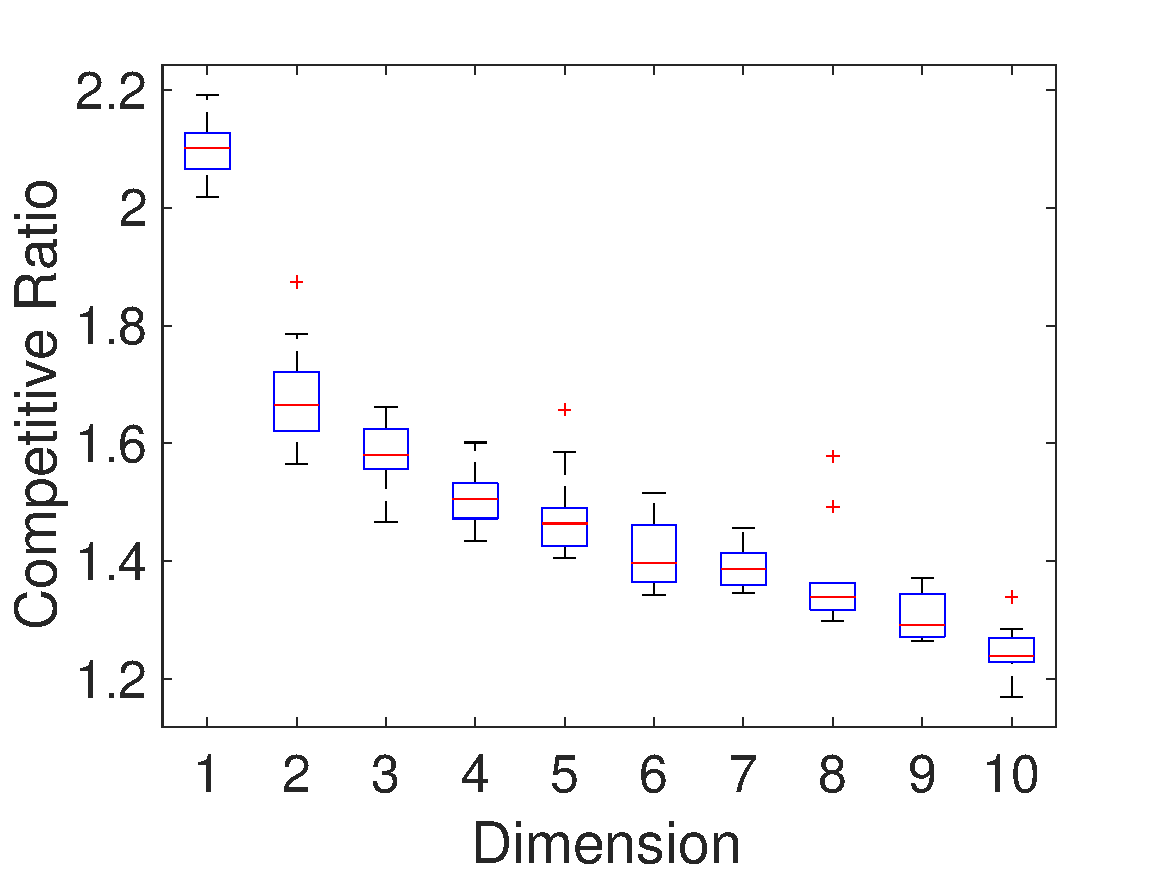
\includegraphics[width=.5\textwidth]{CR_vs_dimension}
	\caption{Competitive ratio against dimension while keeping the diameter of the feasible set constant}
	\label{fig: cr_vs_dim}
\end{figure}
Fig. \ref{fig: cr_vs_dim} shows that, surprisingly, the competitive ratio of Algorithm \ref{alg: online-projection} decreases as the dimension of the problem increases. 

\subsection{Linear cost}
We set $\beta = 0.5$, and $f_t(x) = \| A_t x - y_t\|_2$, where $A_t$ is a random $d \times d$ matrix with fixed condition number (default set to 10), and $y_t \in \mathcal{Y} \subset \mathbb{R}^d$, and the diameter of $\mathcal{Y}$ is fixed (default set to 10). We vary the number of dimension $d$ for the problem, for each dimension, we run 10 trials, the result is shown in Fig. \ref{fig: cr_vs_dim_lin}.
 \begin{figure}[h!]
	\centering
	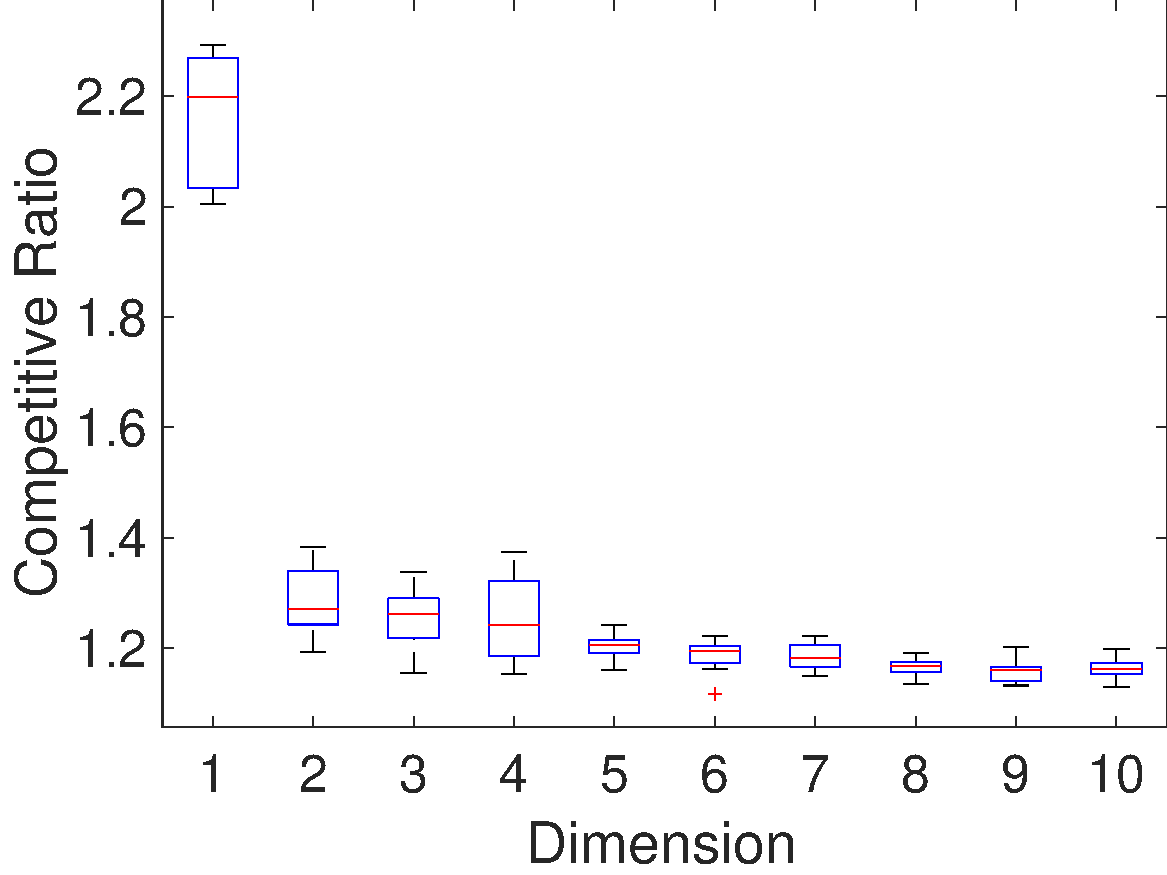
\includegraphics[width=.5\textwidth]{CR_vs_dimension_lin}
	\caption{Competitive ratio against dimension while keeping the diameter of the feasible set constant}
	\label{fig: cr_vs_dim_lin}
\end{figure}

%\section{Concluding remarks}

%\adam{still needs work} In this paper we have introduced a new algorithmic framework, \ouralg\ (\ourack), and used it to (i) break through the $\sqrt{d}$ barrier on the competitive ratio of SOCO, achieving a dimension-free competitive ratio for locally polyhedral cost functions, and (ii) provide the first bounds on dynamic regret in SOCO that do not require the algorithm to use predictions of future cost functions.  \ourack\ is a promising new online optimization framework and we expect that it will be of interest beyond SOCO problems.  Specifically, we expect the idea of projecting onto a carefully chosen level set that balances switching (movement) costs with hitting (stage) costs can be adapted to many other online learning problems.  To that end, it will be important to explore the potential for forms of ``balance'' beyond the primal and dual balance conditions used in this paper.  It will be interesting to see how the appropriate notion of ``balance'' depends on the application and performance metric considered. Further, the development of a stochastic version of \ourack\ is of particular interest, given the prominence and importance of SGD in machine learning applications.  


\bibliography{CR_reference}

\begin{appendix}
\appendix

\section{Proof of Lemma \ref{thm:general_instantaneous}}
\begin{proof}{\textbf{of Lemma \ref{thm:general_instantaneous}}.}
We first state a useful property used in typical OMD analysis. Let $\Omega$ be a convex compact set in $\mathbb{R}^K$, $\psi$ be a convex function on $\Omega$, 
$w'$ be an arbitrary point in $\Omega$, and $x \in \mathbb{R}^K$.
If $w^*=\argmin_{w\in \Omega}\{\inn{w,x}+D_{\psi}(w,w')\}$, then for any $u \in \Omega$,
\begin{align*}
\inn{w^*-u, x}\leq D_{\psi}(u,w')-D_\psi(u,w^*)-D_{\psi}(w^*,w'). 
\end{align*}
This is by the first-order optimality condition of $w^*$ and direct calculations. Applying this to update rule~\eqref{eqn:update_rule_2} we have
\begin{align}
\inn{w_{t+1}^\p-u, \hat{\ell}_t+ a_t} \leq D_{\psi_t}(u,w_{t}^\p)-D_{\psi_t}(u,w_{t+1}^\p)-D_{\psi_t}(w_{t+1}^\p, w_{t}^\p); \label{eqn:apply1}
\end{align}
while applying it to update rule~\eqref{eqn:update_rule_1} and picking $u=w_{t+1}^\p$ we have
\begin{align}
\inn{w_t-w_{t+1}^\p, m_t} \leq D_{\psi_t}(w_{t+1}^\p, w_t^\p)-D_{\psi_t}(w_{t+1}^\p, w_t)-D_{\psi_t}(w_t, w_t^\p).\label{eqn:apply2} 
\end{align}
Now we bound the instantaneous regret as follows:
\begin{align}
&\inn{w_t-u, \hat{\ell}_t}\nonumber \\
&=\inn{w_t-u, \hat{\ell}_t+ a_t}-\inn{w_t, a_t}+\inn{u,  a_t}\nonumber \\
&=\inn{w_t-w_{t+1}^\p, \hat{\ell}_t+a_t}-\inn{w_t, a_t}+\inn{w_{t+1}^\p-u, \hat{\ell}_t+a_t}+\inn{u,   a_t}\nonumber \\
&=\inn{w_t-w_{t+1}^\p, \hat{\ell}_t+a_t-m_t}-\inn{w_t,a_t}+\inn{w_{t+1}^\p-u, \hat{\ell}_t+ a_t}+\inn{w_t-w_{t+1}^\p, m_t}+\inn{u,   a_t} \nonumber \\
&\leq D_{\psi_t}(u,w_{t}^\p)-D_{\psi_t}(u,w_{t+1}^\p)-D_{\psi_t}(w_{t+1}^\p, w_t)-D_{\psi_t}(w_t, w_t^\p)+\inn{u, a_t}, \label{eqn:regret_decomposition}
\end{align}
where last inequality is by the condition $\inn{w_t-w_{t+1}^\p, \hat{\ell}_t+a_t-m_t}-\inn{w_t,a_t}\leq 0$, Eq.~\eqref{eqn:apply1}, and Eq.~\eqref{eqn:apply2}.
\end{proof}

\section{Lemmas for Log-barrier OMD}
\label{section:all_kinds_of_lemmas}

In this section we establish some useful lemmas for update rules~\eqref{eqn:update_rule_1} and~\eqref{eqn:update_rule_2} with log-barrier regularizer,
which are used in the proofs of other theorems.
We start with some definitions.

\begin{definition}
\label{definition:norm}
For any $h \in \mathbb{R}^K$, define norm $\norm{h}_{t,w}=\sqrt{h^\top \nabla^2 \psi_t(w) h}=\sqrt{\sum_{i=1}^K \frac{1}{\eta_{t,i}}\frac{h_i^2}{w_i^2}}$ and its dual norm $\norm{h}_{t,w}^*=\sqrt{h^\top \nabla^{-2} \psi_t(w) h}=\sqrt{\sum_{i=1}^K \eta_{t,i}w_i^2 h_i^2}$.
For some radius $r > 0$, define ellipsoid $\mathcal{E}_{t,w}(r)=\left\{u \in \mathbb{R}^K : \norm{u-w}_{t,w}\leq r \right\}$ . 
\end{definition}

\begin{lemma}
\label{lemma:norm_close}
If $w^\p \in \mathcal{E}_{t,w}(1)$ and $\eta_{t,i}\leq \frac{1}{81}$ for all $i$, then $w_i^\p\in \left[ \frac{1}{2}w_i, \frac{3}{2}w_i \right]$ for all $i$, and also $ 0.9\norm{h}_{t,w} \leq \norm{h}_{t,w^\p} \leq 1.2\norm{h}_{t,w}$ for any $h\in \mathbb{R}^K$. 
\end{lemma}
\begin{proof}
$w^\p\in \mathcal{E}_{t,w}(1)$ implies $\sum_{i=1}^K \frac{1}{\eta_{t,i}}\frac{(w^\p_i-w_i)^2}{w_i^2}\leq 1$. Thus for every $i$, we have $\frac{\abs{w_i^\p-w_i}}{w_i}\leq \sqrt{\eta_{t,i}}\leq \frac{1}{9}$, implying $w_i^\p\in \left[ \frac{8}{9}w_i, \frac{10}{9}w_i \right]\subset\left[ \frac{1}{2}w_i, \frac{3}{2}w_i \right]$. 
Therefore, $\norm{h}_{t,w^\p}
=\sqrt{\sum_{i=1}^K \frac{1}{\eta_{t,i}} \frac{h_i^2}{w^{\p 2}_i}}
\geq \sqrt{\sum_{i=1}^K \frac{1}{\eta_{t,i}}\frac{h_i^2}{\left(\frac{10}{9}w_i\right)^2}}
=0.9\norm{h}_{t,w}$. 
Similarly, we have $\norm{h}_{t,w^\p}\leq 1.2\norm{h}_{t,w}$. 
\end{proof}

\begin{lemma}
\label{lemma:stability}
Let $w_t, w_{t+1}^\p$ follow \eqref{eqn:update_rule_1} and \eqref{eqn:update_rule_2} where $\psi_t$ is the log-barrier with $\eta_{t,i}\leq \frac{1}{81}$ for all $i$. If $\norm{\hat{\ell}_t-m_t+a_t}^*_{t,w_t}\leq \frac{1}{3}$, then $w_{t+1}^\p \in \mathcal{E}_{t,w_t}(1)$. 
\end{lemma}

\begin{proof}
Define $F_{t}(w)=\inn{w, m_t}+D_{\psi_t}(w, w_t^\p)$ and $F_{t+1}^\p(w)=\inn{w, \hat{\ell}_t+a_t}+D_{\psi_t}(w, w_t^\p)$. Then by definition we have $w_t=\argmin_{w\in\Omega}F_{t}(w)$ and $w_{t+1}^\p=\argmin_{w\in\Omega}F_{t+1}^\p(w)$. To show $w_{t+1}^\p\in \mathcal{E}_{t,w_t}(1)$, it suffices to show that for all $u$ on the boundary of $\mathcal{E}_{t,w_t}(1)$, $F^\p_{t+1}(u)\geq F^\p_{t+1}(w_t)$. 

Indeed, using Taylor's theorem, for any $u\in \partial \mathcal{E}_{t,w_t}(1)$, there is an $\xi$ on the line segment between $w_t$ and $u$ such that (let $h\triangleq u-w_t$)
\begin{align*}
F^\p_{t+1}(u)&=F^\p_{t+1}(w_t)+\nabla F^{\p}_{t+1} (w_t)^\top h+ \frac{1}{2}h^\top\nabla^2 F^\p_{t+1}(\xi)h \\
&=F^\p_{t+1}(w_t)+ (\hat{\ell}_t-m_t+a_t)^\top h +\nabla F_t (w_t)^\top h+ \frac{1}{2}h^\top\nabla^2 \psi_t(\xi)h \\
&\geq F^\p_{t+1}(w_t)+ (\hat{\ell}_t-m_t+a_t)^\top h + \frac{1}{2}\norm{h}_{t,\xi}^2 \tag{by the optimality of $w_t$}\\
&\geq F^\p_{t+1}(w_t)+ (\hat{\ell}_t-m_t+a_t)^\top h + \frac{1}{2}\times0.9^2\norm{h}_{t,w_t}^2 \tag{by Lemma \ref{lemma:norm_close}} \\
&\geq F^\p_{t+1}(w_t)- \norm{\hat{\ell}_t-m_t+a_t}^*_{t,w_t} \norm{h}_{t,w_t} + \frac{1}{3}\norm{h}_{t,w_t}^2 \\
&=F^\p_{t+1}(w_t)- \norm{\hat{\ell}_t-m_t+a_t}^*_{t,w_t} + \frac{1}{3} \tag{$\norm{h}_{t,w_t}=1$}\\
&\geq F^\p_{t+1}(w_t). \tag{by the assumption}
\end{align*}
\end{proof}

\begin{lemma}
\label{lemma:stability_under_condition}
Let $w_t, w_{t+1}^\p$ follow \eqref{eqn:update_rule_1} and \eqref{eqn:update_rule_2} where $\psi_t$ is the log-barrier with $\eta_{t,i}\leq \frac{1}{81}$ for all $i$. If $\norm{\hat{\ell}_t-m_t+a_t}^*_{t,w_t}\leq \frac{1}{3}$, then $\norm{w_{t+1}^\p-w_t}_{t,w_t}\leq 3\norm{\hat{\ell}_t-m_t+a_t}_{t,w_t}^*$. 
\end{lemma}
\begin{proof}
Define $F_t(w)$ and $F_{t+1}^\p(w)$ to be the same as in Lemma \ref{lemma:stability}. Then we have 
\begin{align}
F_{t+1}^\p(w_t)-F_{t+1}^\p(w_{t+1}^\p)&=(w_t-w_{t+1}^\p)^\top(\hat{\ell}_t-m_t+a_t) + F_t(w_t)-F_t(w_{t+1}^\p) \nonumber \\
&\leq (w_t-w_{t+1}^\p)^\top(\hat{\ell}_t-m_t+a_t) \nonumber \tag{optimality of $w_t$}\\
&\leq \norm{w_t-w_{t+1}^\p}_{t,w_t}\norm{\hat{\ell}_t-m_t+a_t}_{t,w_t}^*. \label{eqn:direction1}
\end{align}
On the other hand, for some $\xi$ on the line segment between $w_t$ and $w_{t+1}^\p$, we have by Taylor's theorem and the optimality of $w_{t+1}^\p$,
\begin{align}
F_{t+1}^\p(w_t)-F_{t+1}^\p(w_{t+1}^\p)&=\nabla F_{t+1}^\p(w_{t+1}^\p)^\top (w_t-w_{t+1}^\p) + \frac{1}{2}(w_t-w_{t+1}^\p)^\top \nabla^2 F_{t+1}^\p(\xi)(w_t-w_{t+1}^\p) \nonumber \\
&\geq \frac{1}{2}\norm{w_t-w_{t+1}^\p}_{t,\xi}^2 .
\label{eqn:direction2}
\end{align}
Since the condition in Lemma \ref{lemma:stability} holds, $w_{t+1}^\p\in \mathcal{E}_{t,w_t}(1)$, and thus $\xi\in \mathcal{E}_{t,w_t}(1)$. Using again Lemma \ref{lemma:norm_close}, we have 
\begin{align}
\frac{1}{2}\norm{w_t-w_{t+1}^\p}_{t,\xi}^2 \geq \frac{1}{3}\norm{w_t-w_{t+1}^\p}_{t,w_t}^2\label{eqn:direction3}.
\end{align}
Combining \eqref{eqn:direction1}, \eqref{eqn:direction2}, and \eqref{eqn:direction3}, we have $\norm{w_t-w_{t+1}^\p}_{t,w_t}\norm{\hat{\ell}_t-m_t+a_t}_{t,w_t}^* \geq \frac{1}{3}\norm{w_t-w_{t+1}^\p}_{t,w_t}^2$, which leads to the stated inequality. 
\end{proof}

\begin{lemma}
\label{lemma:condition_automatic_hold}
%Let $w_t, w_{t+1}^\p$ follow \eqref{eqn:update_rule_1} and \eqref{eqn:update_rule_2}. 
When the three conditions in Theorem \ref{lemma:MAB_condition} hold, we have $\norm{\hat{\ell}_t-m_t+a_t}^{*}_{t,w_t}\leq \frac{1}{3}$ for either $a_{t,i}=6\eta_{t,i}w_{t,i}(\hat{\ell}_{t,i}-m_{t,i})^2$ or $a_{t,i}=0$.  
\end{lemma}
\begin{proof}
For $a_{t,i}=6\eta_{t,i}w_{t,i}(\hat{\ell}_{t,i}-m_{t,i})^2$, we have
\begin{align*}
\norm{\hat{\ell}_t-m_t+a_t}^{*2}_{t,w_t}
&= \sum_{i=1}^K\eta_{t,i}w_{t,i}^2\big(\hat{\ell}_{t,i}-m_{t,i} + 6\eta_{t,i}w_{t,i}(\hat{\ell}_{t,i}-m_{t,i})^2\big)^2 \\
&=\sum_{i=1}^K\eta_{t,i}w_{t,i}^2(\hat{\ell}_{t,i}-m_{t,i})^2+12\eta_{t,i}^2w_{t,i}^3(\hat{\ell}_{t,i}-m_{t,i})^3 +36\eta_{t,i}^3w_{t,i}^4(\hat{\ell}_{t,i}-m_{t,i})^4\\
&\leq \sum_{i=1}^K \eta_{t,i}w_{t,i}^2(\hat{\ell}_{t,i}-m_{t,i})^2(1+36\eta_{t,i}+324\eta_{t,i}^2) \tag{condition (ii)}\\
&\leq 2\sum_{i=1}^K \eta_{t,i}w_{t,i}^2(\hat{\ell}_{t,i}-m_{t,i})^2 \tag{condition (i)}\\
&\leq 2\times \frac{1}{18}=\frac{1}{9}.\tag{condition (iii)}
\end{align*}
For $a_{t,i}=0$, we have
\begin{align*}
\norm{\hat{\ell}_t-m_t+a_t}^{*2}_{t,w_t}=\norm{\hat{\ell}_t-m_t}^{*2}_{t,w_t}=\sum_{i=1}^K \eta_{t,i}w_{t,i}^2(\hat{\ell}_{t,i}-m_{t,i})^2\leq \frac{1}{18} < \frac{1}{9}. \tag{condition (iii)}
\end{align*}
%When $a_{t,i}=0$,
%\begin{align*}
%\norm{\hat{\ell}_t-m_t+a_t}_{t,w_t}^{*2}= \sum_{i=1}^K \eta_{t,i}w_{t,i}^2(\hat{\ell}_{t,i}-m_{t,i})^2 \leq \frac{1}{18}<\frac{1}{9}. \text{\ \ \ \ \ \ \ \ \ \ \ \ \ \ \ \ \ \ \ \ \ \ \ (condition(iii))} 
%\end{align*}
\end{proof}

\begin{lemma}
\label{lemma:2times_bound}
If the three conditions in Theorem \ref{lemma:MAB_condition} hold, \textsc{Broad-OMD} (with either Option I or II)
satisfies $\frac{1}{2}w_{t,i}\leq w^\p_{t+1,i}\leq \frac{3}{2}w_{t,i}$.
%Let $w_t, w_{t+1}^\p$ follow \eqref{eqn:update_rule_1} and \eqref{eqn:update_rule_2}. If the three conditions in Theorem \ref{lemma:MAB_condition} hold, then $\frac{1}{2}w_{t,i}\leq w^\p_{t+1,i}\leq \frac{3}{2}w_{t,i}$, for either $a_{t,i}=6\eta_{t,i}w_{t,i}(\hat{\ell}_{t,i}-m_{t,i})^2$ or $a_{t,i}=0$.
\end{lemma}
\begin{proof}
This is a direct application of Lemmas \ref{lemma:condition_automatic_hold},  \ref{lemma:stability}, and \ref{lemma:norm_close}.
%It suffices to prove $w_{t+1}^\p \in \mathcal{E}_{t,w_t}(1)$, because if it is true, then
%\begin{align*}
%\norm{w_{t+1}^\p-w_t}_{t,w_t}=\sqrt{\sum_{i=1}^K\frac{1}{\eta_{t,i}}\frac{(w^\p_{t+1,i}-w_{t,i})^2}{w_{t,i}^2}}\leq 1, 
%\end{align*}
%which implies $\frac{\abs{w_{t+1,i}^\p-w_{t,i}}}{w_{t,i}}\leq \sqrt{\eta_{t,i}}\leq \frac{1}{2}$. Thus, $w_{t+1,i}^\p \in [\frac{1}{2}w_{t,i}, \frac{3}{2}w_{t,i}]$.

%Since we assume the three conditions in Theorem \ref{lemma:MAB_condition} hold, $w_{t+1}^\p \in \mathcal{E}_{t,w_t}(1)$ can be proved by applying Lemma \ref{lemma:condition_automatic_hold} and Lemma \ref{lemma:stability} back to back.

\end{proof}

\begin{lemma}
\label{lemma:2times_bound_another}
For the MAB problem, if the three conditions in Theorem \ref{lemma:MAB_condition} hold, \textsc{Broad-OMD} (with either Option I or II)
satisfies $\frac{1}{2}w_{t,i}\leq w^\p_{t,i}\leq \frac{3}{2}w_{t,i}$.
\end{lemma}
\begin{proof}
It suffices to prove $w_{t}^\p \in \mathcal{E}_{t,w_t}(1)$ by Lemma~\ref{lemma:norm_close}.
Since we assume that the three conditions in Theorem \ref{lemma:MAB_condition} hold and $w_t\in \Delta_K$, we have $\norm{m_t}_{t,w_t}^*=\sqrt{\sum_{i=1}^K \eta_{t,i}w_{t,i}^2m_{t,i}^2}\leq \sqrt{\frac{1}{162}\sum_{i=1}^K w_{t,i}^2}\leq \sqrt{\frac{1}{162}}< \frac{1}{3}$. This implies $w_{t}^\p \in \mathcal{E}_{t,w_t}(1)$ by a similar arguments as in the proof of Lemma~\ref{lemma:stability} (one only needs to replace $F_{t+1}^\p(w)$ there by $G(w)\triangleq D_{\psi_t}(w,w_t^\p)$ and note that $w_t^\p=\argmin_{w\in \Delta_K}G(w)$).
\end{proof}


%\begin{lemma}
%\label{lemma:stability_game}
%For MAB problems, if the three conditions in Theorem \ref{lemma:MAB_condition} hold, then \textsc{Broad-OMD} with $a_{t,i}=\mathbf{0}$ and fixed learning rate $\eta$ guarantees $\norm{w_{t+1}-w_t}_1 = \mathcal{O}(\eta)$ for all $t$.  
%\end{lemma}
%\begin{proof}
%By Lemma \ref{lemma:condition_automatic_hold} and \ref{lemma:stability_under_condition}, we have $\norm{w_t-w_{t+1}^\p}_{t,w_t}\leq 3\norm{\hat{\ell}_t-m_t}_{t,w_t}^*$, which implies
%\begin{align*}
%\frac{1}{\eta}\frac{(w_{t,j}-w_{t+1,j}^\p)^2}{w_{t,j}^2}\leq \sum_{i=1}^K\frac{1}{\eta}\frac{(w_{t,i}-w_{t+1,i}^\p)^2}{w_{t,i}^2}\leq 3\eta\sum_{i=1}^K  w_{t,i}^2(\hat{\ell}_{t,i}-m_{t,i})^2\leq 3\eta\times 9. 
%\end{align*}
%Therefore, $\abs{w_{t,j}-w_{t+1,j}^\p} = \mathcal{O}(\eta w_{t,j})$. We can use similar techniques in Lemma \ref{lemma:condition_automatic_hold} and \ref{lemma:stability_under_condition} to prove $\norm{w_{t+1}-w_{t+1}^\p}_{t,w_{t+1}^\p}\leq 3\norm{m_{t+1}}_{t,w_{t+1}^\p}^*$, and thus  $\abs{w_{t+1,j}^\p-w_{t+1,j}}=\mathcal{O}(\eta w_{t+1,j}^\p)=\mathcal{O}(\eta w_{t,j})$. Thus, $\abs{w_{t,j}-w_{t+1,j}}=\mathcal{O}(\eta w_{t,j})$, which implies $\norm{w_t-w_{t+1}}_1=\mathcal{O}(\eta)$. 
%\end{proof}

\section{Proof of Theorem \ref{lemma:MAB_condition} and Corollary~\ref{cor:clear_corollary}}
%To prove Theorem \ref{lemma:MAB_condition}, we need some definitions and lemmas established in Section~\ref{section:all_kinds_of_lemmas}. 

\begin{proof}{\textbf{of Theorem \ref{lemma:MAB_condition}}.}
We first prove Eq.~\eqref{eqn:condition1} holds: by Lemmas \ref{lemma:condition_automatic_hold} %, we have $\norm{\hat{\ell}_t-m_t+a_t}^{*}_{t,w_t}\leq \frac{1}{3}$. Then by
and \ref{lemma:stability_under_condition}, we have
\begin{align*}
\inn{w_t-w_{t+1}^\p, \hat{\ell}_t-m_t+ a_t}
&\leq \norm{w_t-w_{t+1}^\p}_{t,w_t}\norm{\hat{\ell}_t-m_t+a_t}_{t,w_t}^*\\
&\leq 3\norm{\hat{\ell}_t-m_t+a_t}_{t,w_t}^{*2}\\
&\leq 3\sum_{i=1}^K \eta_{t,i}w_{t,i}^2(\hat{\ell}_{t,i}-m_{t,i})^2(1+36\eta_{t,i}+324\eta_{t,i}^2) \\
&\leq 6\sum_{i=1}^K \eta_{t,i}w_{t,i}^2(\hat{\ell}_{t,i}-m_{t,i})^2 = \inn{w_t, a_t},
\end{align*}
where the last two inequalities are by the same calculations done in the proof of Lemma~\ref{lemma:condition_automatic_hold}.
%where $C=6$. With our choice of $C$ and $\eta_{t,i}$, we have $3(1+6\eta_{t,i}C+9\eta_{t,i}^2C^2)\leq 3\left(1+6\times\frac{6}{162}+9\times \left(\frac{6}{162}\right)^2\right)\leq C$. Therefore, the last expression is further bounded by $\sum_{i=1}^K C\eta_{t,i}w_{t,i}^2(\hat{\ell}_{t,i}-m_{t,i})^2$, which is equal to $\inn{w_t, a_t}$. 

Since Eq.~\eqref{eqn:condition1} holds, using Lemma~\ref{thm:general_instantaneous} we have (ignoring non-positive terms $-A_t$'s),
\begin{align}
\sum_{t=1}^T\inn{w_t-u, \hat{\ell}_t}&\leq \sum_{t=1}^T\left(D_{\psi_t}(u,w_t^\p)-D_{\psi_t}(u,w^\p_{t+1})\right)+\sum_{t=1}^T\inn{u,a_t}\nonumber \\
&\leq D_{\psi_1}(u, w_1^\p) + \sum_{t=1}^{T}\left( D_{\psi_{t+1}}(u, w^\p_{t+1})-D_{\psi_{t}}(u, w^\p_{t+1}) \right)+\sum_{t=1}^T\inn{u,a_t}.\label{eqn:some_intermediate}
\end{align}
In the last inequality, we add a term $D_{\psi_{T+1}}(u, w_{T+1}^\p) \geq 0$ artificially. As mentioned, $\psi_{T+1}$, defined in terms of $\eta_{T+1,i}$, never appears in the \textsc{Broad-OMD} algorithm. We can simply pick any $\eta_{T+1,i} > 0$ for all $i$ here. This is just to simplify some analysis later. 

The first term in \eqref{eqn:some_intermediate} can be bounded by the optimality of $w_1^\p$:
\begin{align*}
D_{\psi_1}(u, w_1^\p)&=\psi_1(u)-\psi_1(w_1^\p)-\inn{\nabla\psi_1(w_1^\p), u-w_1^\p}\\
&\leq \psi_1(u)-\psi_1(w_1^\p)=\sum_{i=1}^K \frac{1}{\eta_{1,i}}\ln\frac{w_{1,i}^\p}{u_i}.
\end{align*}
%where the inequality is because $w_1^\p$ is the minimizer of $\psi_1$. 
The second term, by definition, is
\begin{align*}
\sum_{t=1}^{T}\sum_{i=1}^K \left(\frac{1}{\eta_{t+1,i}}-\frac{1}{\eta_{t,i}}\right) h\left(\frac{u_i}{w_{t+1,i}^\p}\right). 
\end{align*}
Plugging the above two terms into \eqref{eqn:some_intermediate} finishes the proof.
\end{proof}

\begin{proof}{\textbf{of Corollary~\ref{cor:clear_corollary}}.}
We first check the three conditions in Theorem~\ref{lemma:MAB_condition} under our choice of $\eta_{t,i}$ and $\hat{\ell}_{t,i}$: $\eta_{t,i}=\eta=\frac{1}{162K_0}\leq \frac{1}{162}$; $w_{t,i}\abs{\hat{\ell}_{t,i}-m_{t,i}}=\abs{\ell_{t,i}-m_{t,i}}\mathbbm{1}\{i\in b_t\} \leq 2<3$; 
$\sum_{i=1}^K \eta_{t,i}w_{t,i}^2(\hat{\ell}_{t,i}-m_{t,i})^2=\frac{1}{162K_0}\sum_{i=1}^K (\ell_{t,i}-m_{t,i})^2\mathbbm{1}\{i\in b_t\} \leq \frac{4}{162} < \frac{1}{18}$. 
%(in the MAB case, $\sum_{i=1}^K \eta_{t,i}w_{t,i}^2(\hat{\ell}_{t,i}-m_{t,i})^2=\eta_{t,i_t}(\ell_{t,i_t}-m_{t,i_t})^2\leq \frac{1}{162}\times 3^2=\frac{1}{18}$). 
Applying Theorem~\ref{lemma:MAB_condition} we then have 
\begin{align*}
\sum_{t=1}^T \inn{w_t-u, \hat{\ell}_t}\leq \sum_{i=1}^K  \frac{\ln\frac{w^\p_{1,i}}{u_i}}{\eta}  +\sum_{t=1}^T \inn{u,a_t}.
\end{align*}
As mentioned, if we let $u=b^*$, then $\ln \frac{w_{1,i}^\p}{u_i}$
becomes infinity for those $i\notin b^*$. Instead, we let $u=\left(1-\frac{1}{T}\right)b^* + \frac{1}{T}w_1^\p$. With this choice of $u$, we have $\frac{w_{1,i}^\p}{u_i}\leq \frac{w_{1,i}^\p}{\frac{1}{T}w_{1,i}^\p}=T$. Plugging $u$ into the above inequality and rearranging, we get 
\begin{align}
\sum_{t=1}^T \inn{w_t-b^*, \hat{\ell}_t}\leq \frac{K\ln T}{\eta}+\sum_{t=1}^T \inn{b^*,a_t}+B,  \label{eqn:sb_corollary}
\end{align}
where $B\triangleq \frac{1}{T}\sum_{t=1}^T \inn{-b^*+w_1^\p, \hat{\ell}_t+a_t}$. 

Now note that $\mathbb{E}_{b_t}[a_{t,i}]=6\eta (\ell_{t,i}-m_{t,i})^2=\mathcal{O}(\eta)$ and $\mathbb{E}_{b_t}[\hat{\ell}_{t,i}]=\ell_{t,i}=\mathcal{O}(1)$ for all $i$. Thus, $\mathbb{E}[B]=\mathbb{E}\left[\frac{1}{T}\sum_{t=1}^T \inn{-b^*+w_1^\p, \mathbb{E}_{b_t}[\hat{\ell}_t+a_t]}\right] \leq \mathbb{E}\left[\frac{1}{T}\sum_{t=1}^T \norm{-b^*+w_1^\p}_1 \norm{\mathbb{E}_{b_t}[\hat{\ell}_t+a_t]}_\infty\right] = \mathcal{O}(K_0)$. Taking expectation on both sides of \eqref{eqn:sb_corollary}, we have 
\begin{align*}
\mathbb{E}\left[\sum_{t=1}^T b_t^\top \ell_t  - \sum_{t=1}^T b^{*\top} \ell_t \right] \leq \frac{K\ln T}{\eta} + 6\eta\mathbb{E}\left[\sum_{t=1}^T \sum_{i\in b^*}^K (\ell_{t,i}-m_{t,i})^2\right] + \mathcal{O}(K_0). 
\end{align*}
%One can verify that in the MAB case, the last term can be $\mathcal{O}(1)$ because now $b^*, w_1^\p \in \Delta_K$.  
\end{proof}

\section{Proof of Theorem \ref{cor:variance_bound}}
\begin{proof}{\textbf{of Theorem \ref{cor:variance_bound}}.}
As in \cite{hazan2011better}, 
for the rounds we perform uniform sampling we do not update $w_t^\p$. 
Let $\mathcal{S}$ be the set of rounds of uniform sampling. %Then in all other rounds the learner is essentially running an untouched \textsc{Broad-OMD}. Therefore, we can use Corollary \ref{cor:clear_corollary} to bound the regret. By Corollary \ref{cor:clear_corollary}, 
Then for the other rounds we can apply Corollary \ref{cor:clear_corollary} to arrive at
\begin{align}
\mathbb{E}\left[\sum_{t\in [T]\backslash \mathcal{S}} \ell_{t,i_t}-\ell_{t,i^*} \right]\leq \frac{K\ln T}{\eta} + 6\eta \mathbb{E}\left[\sum_{t\in [T]\backslash \mathcal{S}}(\ell_{t,i^*}-\tilde{\mu}_{t-1,i^*})^2\right] + \mathcal{O}(1). \label{eqn:regret_bound:a_t_neq_0_another} 
\end{align}
The second term can be bounded as follows: 
\begin{align}
&\mathbb{E}\left[\sum_{t\in [T]\backslash \mathcal{S}} (\ell_{t,i^*}-\tilde{\mu}_{t-1,i^*})^2\right]\leq \mathbb{E}\left[\sum_{t=2}^T (\ell_{t,i^*}-\tilde{\mu}_{t-1,i^*})^2\right] \nonumber \\
&\leq 3\sum_{t=2}^T(\ell_{t,i^*}-\mu_{t,i^*})^2+3\sum_{t=2}^T(\mu_{t,i^*}-\mu_{t-1,i^*})^2 + 3\mathbb{E}\left[\sum_{t=2}^T(\mu_{t-1,i^*}-\tilde{\mu}_{t-1,i^*})^2\right].\label{eqn:decompose_three}
\end{align}
The first and the third terms in \eqref{eqn:decompose_three} can be bounded using Lemma 10 and 11 of \citep{hazan2011better} respectively, and they are both of order $\mathcal{O}(Q_{T,i^*}+1)$ if we pick $M=\Theta(\ln T)$. The second term in \eqref{eqn:decompose_three} can be bounded by a constant by Lemma \ref{lemma:second_Q_term}. Thus second term in \eqref{eqn:regret_bound:a_t_neq_0_another}  can be bounded by $\mathcal{O}\left(\eta (Q_{T,i^*}+1)\right)$. Finally, note that $\mathbb{E}\left[\sum_{t=1}^T \ell_{t,i_t}-\ell_{t,i^*} \right]\leq\mathbb{E}\left[\sum_{t\in [T]\backslash \mathcal{S}} \ell_{t,i_t}-\ell_{t,i^*} \right]+2\mathbb{E}[\abs{\mathcal{S}}]$ and that $\mathbb{E}[\abs{\mathcal{S}}]=\mathcal{O}\left(\sum_{t=1}^T \frac{MK}{t}\right)=\mathcal{O}\left(MK\ln T\right)=\mathcal{O}\left(K(\ln T)^2\right)$. Combining everything, we get 
\begin{align*}
\mathbb{E}\left[\sum_{t=1}^T \ell_{t,i_t}-\ell_{t,i^*} \right]=\mathcal{O}\left( \frac{K\ln T}{\eta} + \eta Q_{T,i^*} + K(\ln T)^2\right).
\end{align*}
\end{proof}

\begin{lemma}
\label{lemma:second_Q_term}
For any $i$, $\sum_{t=2}^T (\mu_{t,i}-\mu_{t-1,i})^2=\mathcal{O}(1)$. 
\end{lemma}
\begin{proof}
By definition, \sloppy$\absolute{\mu_{t,i}-\mu_{t-1,i}}=\absolute{\frac{1}{t}\sum_{s=1}^t \ell_{s,i}-\frac{1}{t-1}\sum_{s=1}^{t-1} \ell_{s,i}}=\absolute{\frac{1}{t}\ell_{t,i}-\frac{1}{t(t-1)}\sum_{s=1}^{t-1}\ell_{s,i}}\leq \absolute{\frac{1}{t}\ell_{t,i}}+\absolute{\frac{1}{t(t-1)}\sum_{s=1}^{t-1}\ell_{s,i}}\leq \frac{2}{t}$. Therefore, $\sum_{t=2}^T (\mu_{t,i}-\mu_{t-1,i})^2\leq \sum_{t=2}^T \frac{4}{t^2}=\mathcal{O}(1)$. 
\end{proof}

\section{Proof of Theorem \ref{thm:path_length}}
We first state a useful lemma.
\begin{lemma}
\label{lemma:bound_ni}
Let $n_i$ be such that $\eta_{T+1,i}=\kappa^{n_i}\eta_{1,i}$, i.e., the number of times the learning rate of arm $i$ changes in \textsc{Broad-OMD+}. Then $n_i\leq \log_2 T$, and $\eta_{t,i}\leq 5\eta_{1,i}$ for all $t,i$.  
\end{lemma}
\begin{proof}
Let $t_1, t_2, \ldots, t_{n_i}\in [T]$ be the rounds the learning rate for arm $i$ changes (i.e., $\eta_{t+1,i}=\kappa \eta_{t,i}$ for $t=t_1, \ldots, t_{n_i}$). 
By the algorithm, we have 
\begin{align*}
KT\geq \frac{1}{\bar{w}_{t_{n_i},i}}>\rho_{t_{n_i},i}>2\rho_{t_{n_i-1},i}>\cdots>2^{n_i-1}\rho_{t_1,i}=2^{n_i}K. 
\end{align*}
Therefore, $n_i\leq \log_2 T$. And we have $\eta_{t,i}\leq \kappa^{\log_2 T}\eta_{1,i}=e^{\frac{\log_2 T}{\ln T}}\eta_{1,i}\leq 5\eta_{1,i}$.
\end{proof}




\begin{proof}{\textbf{of Theorem \ref{thm:path_length}}.}
Again, we verify the three conditions stated in Theorem \ref{lemma:MAB_condition}. By Lemma \ref{lemma:bound_ni}, $\eta_{t,i}\leq 5\eta\leq 5\times\frac{1}{810}=\frac{1}{162}$; also, $w_{t,j}\absolute{\hat{\ell}_{t,j}-m_{t,j}}=w_{t,j}\absolute{\frac{(\ell_{t,j}-m_{t,j})\mathbbm{1}\{i_t=j\}}{\bar{w}_{t,j}}}\leq w_{t,j}\absolute{\frac{2}{w_{t,j}\left(1-\frac{1}{T}\right)}}\leq 3$ because we assume $T\geq 3$; finally, $
\sum_{j=1}^K \eta_{t,j}w_{t,j}^2(\hat{\ell}_{t,j}-m_{t,j})^2=\eta_{t,i_t}w_{t,i_t}^2(\hat{\ell}_{t,i_t}-m_{t,i_t})^2\leq \frac{1}{162}\times 3^2=\frac{1}{18}$.

Let $\tau_j$ denote the last round the learning rate for arm $j$ is updated, that is, $\tau_j\triangleq \max\{t\in [T]: \eta_{t+1,j}=\kappa\eta_{t,j} \}$. 
We assume that the learning rate is updated at least once so that $\tau_j$ is well defined, otherwise one can verify that the bound is trivial.
For any arm $i$ to compete with, let 
$u=\left(1-\frac{1}{T}\right)\mathbf{e}_{i}+\frac{1}{T}w_1^\p
=\left(1-\frac{1}{T}\right)\mathbf{e}_{i}+\frac{1}{KT}\mathbf{1}$, which guarantees $\frac{w_{1,i}^\p}{u_i}\leq T$. Applying Theorem \ref{lemma:MAB_condition}, with $B\triangleq \frac{1}{T}\sum_{t=1}^T \inn{-\mathbf{e}_{i}+w^\p_{1}, \hat{\ell}_t+a_t}$ we have
\begin{align}
\sum_{t=1}^T\inn{w_t, \hat{\ell}_t}-\hat{\ell}_{t,i}&\leq \frac{K\ln T}{\eta} + \sum_{t=1}^{T}\sum_{j=1}^K\left(\frac{1}{\eta_{t+1,j}}-\frac{1}{\eta_{t,j}}\right)h\left(\frac{u_{j}}{w_{t+1,j}^\p}\right)+\sum_{t=1}^T a_{t,i}+B\nonumber \\
&\leq \frac{K\ln T}{\eta} + \left(\frac{1}{\eta_{\tau_i+1,i}}-\frac{1}{\eta_{\tau_i,i}}\right)h\left(\frac{u_{i}}{w_{\tau_i+1,i}^\p}\right)+\sum_{t=1}^T a_{t,i}+B\nonumber \\
&\leq \frac{K\ln T}{\eta} + \frac{1-\kappa}{\eta_{\tau_i+1,i}}h\left(\frac{u_{i}}{w_{\tau_i+1,i}^\p}\right)+\sum_{t=1}^T a_{t,i}+B\nonumber \\
&\leq \frac{K\ln T}{\eta} - \frac{1}{5\eta \ln T}h\left(\frac{u_{i}}{w_{\tau_i+1,i}^\p}\right)+\sum_{t=1}^T a_{t,i}+B,  \label{eqn:quasi_regret_bound1}
\end{align}
where the last inequality is by Lemma~\ref{lemma:bound_ni} and the fact $\kappa-1 \geq \frac{1}{\ln T}$. Now we bound the second and the third term in \eqref{eqn:quasi_regret_bound1} separately. 
\begin{enumerate}
\item For the second term,  by Lemma \ref{lemma:2times_bound} and $T \geq 3$ we have
\begin{align*}
\frac{u_{i}}{w^\p_{\tau_i+1,i}} \geq \frac{1-\frac{1}{T}}{ \frac{3}{2}w_{\tau_i, i} }\geq \frac{\left(1-\frac{1}{T}\right)^2}{\frac{3}{2}\bar{w}_{\tau_i,i}} =\frac{\left(1-\frac{1}{T}\right)^2}{\frac{3}{2}}\times \frac{\rho_{T+1,i}}{2}\geq \frac{\rho_{T+1,i}}{8} \geq \frac{4K}{8} \geq 1.
\end{align*}
Noting that $h(y)$ is an increasing function when $y\geq 1$, we thus have
\begin{align}
h\left(\frac{u_{i}}{w^\p_{\tau_i+1,i}}\right)\geq h\left(\frac{\rho_{T+1,i}}{8}\right)
=\frac{\rho_{T+1,i}}{8}-1-\ln\left(\frac{\rho_{T+1,i}}{8}\right)\geq \frac{\rho_{T+1,i}}{8}-1-\ln\left(\frac{KT}{4}\right). \label{eqn:path_length_second_term}
\end{align}

\item For the third term, we proceed as
\begin{align}
\sum_{t=1}^T a_{t,i} &= 6\sum_{t=1}^T \eta_{t,i}w_{t,i}(\hat{\ell}_{t,i}-m_{t,i})^2\leq 90\eta \sum_{t=1}^T \abs{\hat{\ell}_{t,i}-m_{t,i}}  \nonumber \\
&\leq 90\eta\left(\max_{t\in[T]}\frac{1}{\bar{w}_{t,i}}\right) \sum_{t=1}^{T}  \abs{\ell_{t,i}-\ell_{t-1,i}} \leq 90\eta\rho_{T+1,i} V_{T,i}, \label{eqn:path_length_third_term}
\end{align}
where in the first inequality, we use $w_{t,i}\abs{\hat{\ell}_{t,i}-m_{t,i}}\leq 3$ and $\eta_{t,i}\leq 5\eta$; in the second inequality, we do a similar calculation as in Eq.~\eqref{eqn:path_length_trick} (only replacing $w_{t,i}$ by $\bar{w}_{t,i}$); and in the last inequality, we use the fact $\frac{1}{\bar{w}_{t,i}}\leq \rho_{T+1,i}$ for all $t\in [T]$
by the algorithm.
\end{enumerate}
Combining Eq.~\eqref{eqn:path_length_second_term} and Eq.~\eqref{eqn:path_length_third_term} and using the fact $\frac{1+\ln\left(\frac{KT}{4}\right)}{5\ln T}\leq K\ln T$, we continue from Eq.~\eqref{eqn:quasi_regret_bound1} to arrive at
\begin{align}
\sum_{t=1}^T \inn{w_t, \hat{\ell}_t}-\hat{\ell}_{t,i}\leq \frac{2K\ln T}{\eta}+ \rho_{T+1,i}\left( \frac{-1}{40\eta\ln T} +90\eta V_{T,i} \right) +B,  \label{eqn:quasi_regret_bound2}
\end{align}
We are almost done here, but note that the left-hand side of \eqref{eqn:quasi_regret_bound2} is not the desired regret. What we would like to bound is
\begin{align}
\sum_{t=1}^T \inn{\bar{w}_t, \hat{\ell}_t} - \sum_{t=1}^T \hat{\ell}_{t,i}=\sum_{t=1}^T \inn{\bar{w}_t-w_t, \hat{\ell}_t}+ \sum_{t=1}^T\left(\inn{w_t, \hat{\ell}_t}-\hat{\ell}_{t,i}\right), \label{eqn:quasi_regret_bound3}
\end{align}
where the second summation on the right-hand side is bounded by Eq.~\eqref{eqn:quasi_regret_bound2}.
The first term can be written as $\sum_{t=1}^T \inn{-\frac{1}{T}w_t+\frac{1}{KT}\mathbf{1}, \hat{\ell}_t}$. Note that$
\frac{1}{T}\sum_{t=1}^T\inn{-w_t, \hat{\ell}_t}\leq \frac{1}{T}\sum_{t=1}^T\abs{\inn{w_t,\hat{\ell}_t-m_t}}+\frac{1}{T}\sum_{t=1}^T\abs{\inn{w_t, m_t}} \leq 3 + 1=4$, and
$
\mathbb{E}\left[\frac{1}{T}\sum_{t=1}^T \inn{\frac{1}{K}\mathbf{1},\hat{\ell}_{t}}\right]=\frac{1}{T}\sum_{t=1}^T \inn{\frac{1}{K}\mathbf{1},\ell_t}\leq 1. $
Therefore, taking expectation on both sides of \eqref{eqn:quasi_regret_bound3}, we get 
\begin{align*}
\mathbb{E}\left[\sum_{t=1}^T \ell_{t,i_t} \right] - \sum_{t=1}^T \ell_{t,i} \leq \frac{2K\ln T}{\eta} + \mathbb{E}[\rho_{T+1,i}]\left( \frac{-1}{40\eta\ln T} +90\eta V_{T,i} \right) + \mathcal{O}(1),   
\end{align*}
because $\mathbb{E}[B]$ is also $\mathcal{O}(1)$ as proved in Corollary~\ref{cor:clear_corollary}. 
\end{proof}

\section{Proofs of Lemma \ref{lemma:simple_lemma} and Theorem \ref{lemma:second_order_regret_bound}}

\begin{proof}{\textbf{of Lemma \ref{lemma:simple_lemma}}.}
By the same arguments as in the proof of Lemma~\ref{thm:general_instantaneous}, we have
\begin{align*}
\inn{w_{t+1}^\p-u, \hat{\ell}_t} \leq D_{\psi_t}(u,w_{t}^\p)-D_{\psi_t}(u,w_{t+1}^\p)-D_{\psi_t}(w_{t+1}^\p, w_{t}^\p); 
\end{align*}
and 
\begin{align*}
\inn{w_t-w_{t+1}^\p, m_t} \leq D_{\psi_t}(w_{t+1}^\p, w_t^\p)-D_{\psi_t}(w_{t+1}^\p, w_t)-D_{\psi_t}(w_t, w_t^\p).
\end{align*}
Therefore, by expanding the instantaneous regret, we have
\begin{align*}
&\inn{w_t-u, \hat{\ell}_t}\nonumber \\
&=\inn{w_t-w_{t+1}^\p, \hat{\ell}_t-m_t}+\inn{w_{t+1}^\p-u, \hat{\ell}_t}+\inn{w_t-w_{t+1}^\p, m_t} \nonumber \\
&\leq \inn{w_t-w_{t+1}^\p, \hat{\ell}_t-m_t} + D_{\psi_t}(u,w_{t}^\p)-D_{\psi_t}(u,w_{t+1}^\p)-D_{\psi_t}(w_{t+1}^\p, w_t)-D_{\psi_t}(w_t, w_t^\p). 
\end{align*}
\end{proof}
\begin{proof}{\textbf{of Theorem \ref{lemma:second_order_regret_bound}}.}
Applying Lemma \ref{lemma:simple_lemma}, we have 
\begin{align*}
\sum_{t=1}^T\inn{w_t-u, \hat{\ell}_t} &\leq \sum_{t=1}^T \left(D_{\psi_t}(u,w_{t}^\p)-D_{\psi_t}(u,w_{t+1}^\p)+\inn{w_t-w_{t+1}^\p, \hat{\ell}_t-m_t}-A_t\right) \\
&\leq \sum_{i=1}^K \frac{\ln \frac{w_{1,i}^\p}{u_i}}{\eta} +\sum_{t=1}^T \inn{w_t-w_{t+1}^\p, \hat{\ell}_t-m_t}-A_t .
\end{align*}
%The proof of the inequality
%\begin{align*}
%\sum_{t=1}^T D_{\psi_t}(u,w_{t}^\p)-D_{\psi_t}(u,w_{t+1}^\p) \leq \sum_{i=1}^K \left( \frac{\ln \frac{w_{1,i}^\p}{u_i}}{\eta_{1,i}} + \sum_{t=1}^T \left(\frac{1}{\eta_{t+1,i}}-\frac{1}{\eta_{t,i}}\right)h\left(\frac{u_i}{w_{t+1,i}^\p}\right) \right)
%\end{align*}
%is the same as in Lemma \ref{lemma:MAB_condition}. By the non-decreasing learning rate assumption and the fact that $h(\cdot)$ is positive, we can discard $\sum_{t=1}^T \left(\frac{1}{\eta_{t+1,i}}-\frac{1}{\eta_{t,i}}\right)h\left(\frac{u_i}{w_{t+1,i}^\p}\right)$. For the other term, we have 
For the second term, using Lemma \ref{lemma:condition_automatic_hold} and \ref{lemma:stability_under_condition} we bound $\inn{w_t-w_{t+1}^\p, \hat{\ell}_t-m_t}$ by
\begin{align*}
\norm{w_t-w_{t+1}^\p}_{t,w_t}\norm{\hat{\ell}_t-m_t}_{t,w_t}^* 
\leq 3\norm{\hat{\ell}_t-m_t}_{t,w_t}^{*2} = 3\eta\sum_{i=1}^K w_{t,i}^2(\hat{\ell}_{t,i}-m_{t,i})^2
%&= 3\sum_{i=1}^K \eta_{t,i}(\ell_{t,i}-m_{t,i})^2\mathbbm{1}\{i\in b_t\}=3\sum_{i=1}^K \eta_{t,i}b_{t,i}(\ell_{t,i}-m_{t,i})^2
\end{align*}

Finally we lower bound $A_t$ for the MAB case. Note $h(y)=y-1-\ln y\geq \frac{(y-1)^2}{6}$ for $y\in [\frac{1}{2},2]$. By Lemma~\ref{lemma:2times_bound} and \ref{lemma:2times_bound_another}, $\frac{w_{t+1,i}^\p}{w_{t,i}}$ and $\frac{w_{t,i}}{w_{t,i}^\p}$ both belong to $[\frac{1}{2},2]$. Therefore, 
\begin{align*}
A_t&=D_{\psi_t}(w_{t+1}^\p, w_t)+D_{\psi_t}(w_t, w_t^\p)=\frac{1}{\eta} \sum_{i=1}^K \left(h\left(\frac{w_{t+1,i}^\p}{w_{t,i}}\right) +h\left(\frac{w_{t,i}}{w_{t,i}^\p}\right)\right) \\
&\geq \frac{1}{6\eta} \sum_{i=1}^K \left( \frac{(w_{t+1,i}^\p-w_{t,i})^2}{w_{t,i}^2} + \frac{(w_{t,i}-w_{t,i}^\p)^2}{w_{t,i}^{\p 2}} \right) \\
&\geq \frac{1}{24\eta} \sum_{i=1}^K \left( \frac{(w_{t+1,i}^\p-w_{t,i})^2}{w_{t,i}^2} + \frac{(w_{t,i}-w_{t,i}^\p)^2}{w_{t-1,i}^2} \right), 
\end{align*}
and 
\begin{align*}
\sum_{t=1}^T A_t &\geq \frac{1}{24\eta}\sum_{t=2}^{T}\sum_{i=1}^K\frac{(w_{t,i}^\p-w_{t-1,i})^2}{w_{t-1,i}^2}+\sum_{t=2}^T \sum_{i=1}^K \frac{(w_{t,i}-w_{t,i}^\p)^2}{w_{t-1,i}^2}\geq \frac{1}{48\eta}\sum_{t=2}^T \sum_{i=1}^K \frac{(w_{t,i}-w_{t-1,i})^2}{w_{t-1,i}^2}. 
\end{align*}
\end{proof}

\section{Doubling Trick}
\label{app:doubling_trick}

\begin{algorithm}[t]
\DontPrintSemicolon
\caption{Doubling trick for \textsc{Broad-OMD} with $a_t=\mathbf{0}$}
\label{alg:doubling}
\textbf{Initialize}: $\eta=\frac{1}{162K_0}, T_0=0, t=1.$\\
\For{$\beta=0, 1, \ldots$}{
   $w_{t}^\p=\argmin_{w\in \Omega}\psi_1(w)$ (restart \textsc{Broad-OMD}). \\
   \While{$t\leq T$}{
      Update $w_t$, sample $b_t\sim w_t$, and update $w_{t+1}^\p$ as in \textsc{Broad-OMD} with Option II. \\
      \If{$\sum_{s=T_\beta+1}^{t} \sum_{i=1}^K w_{s,i}^2(\hat{\ell}_{s,i}-m_{s,i})^2 \geq \frac{K\ln T}{3\eta^2}$}{
          $\eta \leftarrow \eta/2$, $T_{\beta+1} \leftarrow t$, $t\leftarrow t+1$. \\
          \textbf{break}.
      }
      $t\leftarrow t+1$. 
   }
}
\end{algorithm}

We include the version of our algorithm with the doubling trick in Algorithm~\ref{alg:doubling}.
For simplicity we still assume the time horizon $T$ is known; the extension to unknown horizon is straightforward. 

\begin{proof}{\textbf{of Theorem \ref{thm:doubling_trick_theorem}}.}
Let $u=\left(1-\frac{1}{T}\right)b^*+\frac{1}{T}w_1^\p$ so that $\ln \frac{w^\p_{1,i}}{u_i} \leq \ln T$.
At some epoch $\beta$, by Theorem~\ref{lemma:second_order_regret_bound}, the break condition, and condition (iii) we have with $\eta_\beta\triangleq\frac{2^{-\beta}}{162K_0}$,
\begin{align*}
\sum_{t= T_\beta+1}^{T_{\beta+1}}\inn{w_t-u, \hat{\ell}_t} &\leq \frac{K\ln T}{\eta_\beta} + 
3\eta_\beta\sum_{t=T_\beta+1}^{T_{\beta+1}}\sum_{i=1}^K w_{t,i}^2(\hat{\ell}_{t,i}-m_{t,i})^2 \\
& \leq  \frac{2K\ln T}{\eta_\beta} + 3\eta_\beta \sum_{i=1}^K w_{T_{\beta+1},i}^2(\hat{\ell}_{T_{\beta+1},i}-m_{T_{\beta+1},i})^2 
= \mathcal{O}\left(\frac{K\ln T}{\eta_\beta}\right).
\end{align*}

Suppose that at time $T$, the algorithm is at epoch $\beta=\beta^*$. Then we have
\[
\sum_{t=1}^T\inn{w_t-u, \hat{\ell}_t}\leq\sum_{\beta=0}^{\beta^*}\mathcal{O}\left( \frac{K\ln T}{\eta_\beta} \right)\leq \sum_{\beta=0}^{\beta^*}\mathcal{O}\left( 2^\beta K_0 K\ln T \right)\leq\mathcal{O}\left(2^{\beta^*}K_0 K\ln T\right).
\]
It remains to bound $\beta^*$.
If $\beta^*=0$ (no restart ever happened), then trivially $\sum_{t= 1}^{T}\inn{w_t-u, \hat{\ell}_t}=\mathcal{O}(K_0 K\ln T)$. 
Otherwise, because epoch $\beta^*-1$ finishes, we have 
\begin{align*}
\sum_{t= T_{\beta^*-1}+1}^{T_{\beta^*}}\sum_{i=1}^K w_{t,i}^2(\hat{\ell}_{t,i}-m_{t,i})^2 \geq \frac{K\ln T}{3(\eta_{\beta^*-1})^2} = \Omega(2^{2\beta^*}K_0^2K\ln T).  
\end{align*}
Combining them, we have 
\begin{align}
\sum_{t=1}^T\inn{w_t-u, \hat{\ell}_t} &\leq \mathcal{O}\left(2^{\beta^*}K_0K\ln T\right)
\leq \mathcal{O}\left( \sqrt{(K\ln T)\sum_{t= T_{\beta^*-1}+1}^{T_{\beta^*}}\sum_{i=1}^K w_{t,i}^2(\hat{\ell}_{t,i}-m_{t,i})^2} \right) \nonumber \\
&\leq \mathcal{O}\left( \sqrt{(K\ln T)\sum_{t= 1}^{T}\sum_{i=1}^K w_{t,i}^2(\hat{\ell}_{t,i}-m_{t,i})^2} \right), \label{eqn:doubling_bound_1}
\end{align}
Combining both cases we have 
\begin{align}
\sum_{t=1}^T\inn{w_t-u, \hat{\ell}_t} \leq \mathcal{O}\left( \sqrt{K\ln T\sum_{t= 1}^{T}\sum_{i=1}^K w_{t,i}^2(\hat{\ell}_{t,i}-m_{t,i})^2} + K_0K\ln T\right).
\end{align}
Now substituting $u$ by its definition and taking expectations, with $B\triangleq \frac{1}{T} \sum_{t=1}^T \inn{-b^*+w_1^\p, \hat{\ell}_{t}}$ we arrive at 
\begin{align*}
\mathbb{E}\left[ \sum_{t=1}^T \inn{b_t-b^*, \ell_t} \right]
&\leq \mathcal{O}\left(\mathbb{E}\left[\sqrt{K\ln T\sum_{t= 1}^{T}\sum_{i=1}^K w_{t,i}^2(\hat{\ell}_{t,i}-m_{t,i})^2}\right]+K_0K\ln T \right)+\mathbb{E}[B] \\
&\leq \mathcal{O}\left(  \sqrt{K\ln T\mathbb{E}\left[\sum_{t= 1}^{T}\sum_{i=1}^K w_{t,i}^2(\hat{\ell}_{t,i}-m_{t,i})^2\right]}+K_0K\ln T \right), 
\end{align*}
where the last inequality uses the fact $\mathbb{E}[B]=\mathcal{O}(K)$ and Jensen's inequality.
\end{proof}


\section{Proofs of Corollary \ref{cor:path_length_bound_1} and Theorem \ref{thm:fast_convergence_theorem}}

\begin{proof}{\textbf{of Corollary~\ref{cor:path_length_bound_1}}.}
We first verify the three conditions in Theorem~\ref{lemma:second_order_regret_bound}: $\eta \leq \frac{1}{162}$ by assumption; $w_{t,i}\absolute{\hat{\ell}_{t,i}-m_{t,i}}=\absolute{(\ell_{t,i}-\ell_{\alpha_i(t),i})\mathbbm{1}\{i_t=i\}}\leq 2<3$; $\eta \sum_{i=1}^K w_{t,i}^2(\hat{\ell}_{t,i}-m_{t,i})^2=\eta w_{t,i_t}^2(\hat{\ell}_{t,i_t}-m_{t,i_t})^2\leq \frac{9}{162}=\frac{1}{18}$. Let $u=\left(1-\frac{1}{T}\right)\mathbf{e}_{i^*} + \frac{1}{T}w_1^\p$, which guarantees $\frac{w_{1,i}^\p}{u_i}\leq T$. By Theorem~\ref{lemma:second_order_regret_bound} and some rearrangement, we have
\begin{align*}
\sum_{t=1}^T \inn{w_t-\mathbf{e}_{i^*}, \hat{\ell}_t}\leq \frac{K\ln T}{\eta}  +3\eta\sum_{t=1}^T\sum_{i=1}^K  w_{t,i}^2(\hat{\ell}_{t,i}-m_{t,i})^2-\sum_{t=1}^T A_t+B, 
\end{align*}
where $B\triangleq \frac{1}{T}\sum_{t=1}^T \inn{-\mathbf{e}_{i^*}+w_1^\p, \hat{\ell}_t}$. To get the stated bound, just note that $\mathbb{E}[B]=\mathcal{O}(1)$,  and replace $\sum_{t=1}^T\sum_{i=1}^K w_{t,i}^2(\hat{\ell}_{t,i}-m_{t,i})^2$ by the upper bound at \eqref{eqn:path_length_calculation_1} and $A_t$ by the lower bound in Theorem~\ref{lemma:second_order_regret_bound}.
\end{proof}

\section{Omitted Details in Section~\ref{subsection:games}}
\label{appendix:game}
Although the generalization to multi-player games is straightforward, for simplicity we only consider two-player zero-sum games.

We first describe the protocol of the game. The game is defined by an unknown matrix $G\in[-1,1]^{M\times N}$
where entry $G(i,j)$ specifies the loss (or reward) for Player 1 (or Player 2) if Player 1 picks row $i$ while Player 2 picks column $j$.
The players play the game repeatedly for $T$ rounds.
At round $t$, Player 1 randomly picks a row $i_t \sim x_t$ for some $x_t \in \Delta_M$
while Player 2 randomly picks a column $j_t \sim y_t$ for some $y_t \in \Delta_N$.
In~\citep{syrgkanis2015fast}, the feedbacks they receive are the vectors $Gy_t$ and $x_t^\top G$ respectively.
As a natural extension to the bandit setting, we consider a setting where the feedbacks are the scalar values $\mathbf{e}_{i_t}^\top Gy_t$
and $x_t^\top G\mathbf{e}_{j_t}$ respectively, that is, the expected loss/reward for the players' own realized actions (over the opponent's randomness). 

It is clear that each player is essentially facing an MAB problem and thus can employ an MAB algorithm.
Specifically, if both players apply Exp3 for example, their expected average strategies converge to a Nash equilibrium at rate $1/\sqrt{T}$.
However, if instead Player 1 applies \textsc{Broad-OMD} configured as in Corollary~\ref{cor:path_length_bound_1},
then her regret has a path-length term that can be bounded as follows:
\begin{align*}
\sum_{i=1}^K \sum_{t=2}^T\left| \mathbf{e}_{i}^\top Gy_t -  \mathbf{e}_{i}^\top Gy_{t-1}\right|
\leq \sum_{i=1}^K \sum_{t=2}^T\left\| \mathbf{e}_{i}^\top G \right\|_\infty \|y_t - y_{t-1}\|_1 \leq K \sum_{t=2}^T \|y_t - y_{t-1}\|_1,
\end{align*}
which is closely related to the negative regret term in Corollary~\ref{cor:path_length_bound_1}
for Player 2 if she also employs the same \textsc{Broad-OMD}.
The cancellation of these terms then lead to faster convergence rate.

\begin{theorem}
\label{thm:fast_convergence_theorem}
For the setting described above, if both players run \textsc{Broad-OMD} configured as in Corollary~\ref{cor:path_length_bound_1} except that $\eta_{t,i}=\eta= (M+N)^{-\frac{1}{4}}T^{-\frac{1}{4}}$, then their expected average strategies converge to Nash equilibriums at the rate of $\tilde{\mathcal{O}}\left((M+N)^{\frac{5}{4}}/T^{\frac{3}{4}}\right)$, that is,
\begin{align*}
\max_{y\in \Delta_N} \mathbb{E}[\bar{x}]^\top Gy \leq \text{\rm Val} + \tilde{\mathcal{O}}((M+N)^{\frac{5}{4}}/T^{\frac{3}{4}}) \quad\text{and}\quad
\min_{x\in \Delta_M}x^\top G\mathbb{E}[\bar{y}] \geq \text{\rm Val} - \tilde{\mathcal{O}}((M+N)^{\frac{5}{4}}/T^{\frac{3}{4}}),
\end{align*}
where $\bar{x}=\frac{1}{T}\sum_{t=1}^T x_t, \bar{y}=\frac{1}{T}\sum_{t=1}^T y_t$ and 
$\text{\rm Val}= \min\limits_{x\in \Delta_M}\max\limits_{y\in \Delta_N} x^\top Gy = \max\limits_{y\in \Delta_N}\min\limits_{x\in \Delta_M} x^\top Gy$.
\end{theorem}

\begin{proof}
As mentioned, Player 1's $V_{T,i}$ is 
\begin{align*}
\sum_{t=1}^T \abs{\ell_{t,i}-\ell_{t-1,i}}=&\sum_{t=1}^T \abs{\mathbf{e}_i^\top Gy_t-\mathbf{e}_i^\top Gy_{t-1}}\leq \sum_{t=1}^T \norm{\mathbf{e}_i^\top G}_\infty \norm{y_t-y_{t-1}}_1\leq \sum_{t=1}^T \norm{y_t-y_{t-1}}_1
\end{align*}
due to the assumption $|G(i,j)|\leq 1$. Therefore, by Corollary \ref{cor:path_length_bound_1}, Player 1's (pseudo) regret is
\begin{align*}
&\max_{x \in \Delta_M} \mathbbm{E}\left[\sum_{t=1}^T x_t^\top G y_t - \sum_{t=1}^T x^\top G y_t \right] \\
&\leq \mathcal{O}\left(\frac{M\ln T}{\eta}\right) + \mathbb{E}\left[6\eta M \sum_{t=1}^T \norm{y_t-y_{t-1}}_1 -\frac{1}{48\eta}\sum_{t=2}^T \sum_{i=1}^M \frac{(x_{t,i}-x_{t-1,i})^2}{x_{t-1,i}^2} \right],%\label{eqn:game_regret_1}
\end{align*}
while Player 2's (pseudo) regret is
\begin{align*}
&\max_{y \in \Delta_N} \mathbbm{E}\left[\sum_{t=1}^T x_T^\top G y - \sum_{t=1}^T x_t^\top G y_t \right] \\
&\leq \mathcal{O}\left(\frac{N\ln T}{\eta}\right) + \mathbb{E}\left[6\eta N \sum_{t=1}^T \norm{x_t-x_{t-1}}_1 -\frac{1}{48\eta}\sum_{t=2}^T \sum_{i=1}^N \frac{(y_{t,i}-y_{t-1,i})^2}{y_{t-1,i}^2} \right].%\label{eqn:game_regret_2}
\end{align*}
%Picking $\eta=\Theta\left( T^{-\frac{1}{3}}(\ln T)^{\frac{1}{3}} \right)$, we can bound the right-hand side of \eqref{eqn:game_regret_1} by $\mathcal{O}(M(\ln T)^{\frac{2}{3}}T^{-\frac{2}{3}})=\tilde{\mathcal{O}}(MT^{-\frac{2}{3}})$. With a similar analysis, we have 
Summing up the above two bounds, and using the following fact (by the inequality $a - b \leq \frac{a^2}{4b}$):
\begin{align*}
\sum_{i=1}^N \left(6\eta M \abs{y_{t,i}-y_{t-1,i}}- \frac{(y_{t,i}-y_{t-1,i})^2}{48\eta y_{t-1,i}^2}\right)\leq 432\eta^3 M^2 \sum_{i=1}^N y_{t-1,i}^2 \leq 432\eta^3 M^2, 
\end{align*}
we get 
\begin{align*}
\max_{y \in \Delta_N}\mathbb{E}[\bar{x}]^\top Gy - \min_{x \in \Delta_M} x^\top G \mathbb{E}[\bar{y}] 
 =\mathcal{O}\left(\frac{(M+N)\ln T}{T\eta} + \eta^3 (M^2+N^2) \right).
\end{align*}
With $\eta=\tilde{\Theta}\left( (M+N)^{-\frac{1}{4}}T^{-\frac{1}{4}}\right)$ the above bound becomes $\tilde{\mathcal{O}}\left((M+N)^{\frac{5}{4}}T^{-\frac{3}{4}}\right)$.
Rearranging then gives
%Note that $\mathbb{E}\left[ \frac{1}{T}\left(\text{Reg}_T^1+\text{Reg}_T^2\right) \right]=\mathbb{E}\left[ \max_{y}\bar{x}^\top Gy -\min_{x}x^\top G\bar{y} \right]$. Using 
%By von Neumann’s minimax theorem, we then have
%\begin{align*}
%\max_{y\in \Delta_N}\min_{x\in \Delta_M}x^\top Gy= \min_{x\in \Delta_M}\max_{y\in \Delta_N} x^\top Gy 
%&\leq \max_{y \in \Delta_N}\mathbb{E}[\bar{x}]^\top Gy \leq \min_{x \in \Delta_M} x^\top G \mathbb{E}[\bar{y}]  + \tilde{\mathcal{O}}((M+N)^{\frac{5}{4}}T^{-\frac{3}{4}}) \\
%&\leq \min_{x\in \Delta_M}\max_{y\in \Delta_N} x^\top Gy + \tilde{\mathcal{O}}((M+N)^{\frac{5}{4}}T^{-\frac{3}{4}}).
%\end{align*}
%This implies that in expectation the two players' average strategies $(\bar{x},\bar{y})$ converges to nearly optimal ones in the rate of $\tilde{\mathcal{O}}((M+N)^{\frac{5}{4}}T^{-\frac{3}{4}})$, because 
\begin{align*}
\max_{y\in\Delta_N} \mathbb{E}[\bar{x}]^\top Gy 
&\leq \min_{x \in \Delta_M} x^\top G \mathbb{E}[\bar{y}]  + \tilde{\mathcal{O}}((M+N)^{\frac{5}{4}}T^{-\frac{3}{4}}), \\
&\leq \min_{x\in \Delta_M}\max_{y\in \Delta_N} x^\top Gy + \tilde{\mathcal{O}}((M+N)^{\frac{5}{4}}T^{-\frac{3}{4}})
= \text{\rm Val} + \tilde{\mathcal{O}}((M+N)^{\frac{5}{4}}T^{-\frac{3}{4}}), 
\end{align*}
and similarly
\begin{align*}
\min_{x\in \Delta_M} x^\top G\mathbb{E}[\bar{y}]
&\geq \max_{y\in\Delta_N} \mathbb{E}[\bar{x}]^\top Gy - \tilde{\mathcal{O}}((M+N)^{\frac{5}{4}}T^{-\frac{3}{4}}) \\
&\geq \max_{y\in \Delta_N}\min_{x\in \Delta_M}x^\top Gy - \tilde{\mathcal{O}}((M+N)^{\frac{5}{4}}T^{-\frac{3}{4}})
= \text{\rm Val} - \tilde{\mathcal{O}}((M+N)^{\frac{5}{4}}T^{-\frac{3}{4}}), 
\end{align*}
completing the proof.
\end{proof}

%\begin{proof}{\textbf{of Theorem~\ref{theorem:better_for_stable}}.}
%Similar to the proof of Theorem~\ref{thm:fast_convergence_theorem}, we have by Corollary \ref{cor:path_length_bound_1}, 
%\begin{align*}
%\mathbbm{E}\left[ \text{Reg}_T^1 \right] &=\mathcal{O}\left(\frac{M\ln T}{\eta} + \eta M \mathbb{E}\left[\sum_{t=1}^T \norm{y_t-y_{t-1}}_1\right]  \right).
%\end{align*}
%By our assumption, the bounded is further bounded by $\tilde{\mathcal{O}}\left( \frac{M}{\eta}+\eta MT\kappa \right)$. Selecting the optimal $\eta$ we get the desired bound. 
%\end{proof}

As shown by the theorem, we obtain convergence rate faster than $1/\sqrt{T}$,
but still slower than the $1/T$ rate compared to the full-information setup of~\citep{rakhlin2013optimization, syrgkanis2015fast},
due to the fact that we only have first-order instead of second-order path-length bound.

Note that~\citet{rakhlin2013optimization} also studies two-player zero-sum games with bandit feedback
but with an unnatural restriction that in each round the players play the same strategy for four times.
\citet{foster2016learning} greatly weakened the restriction, but their algorithm only converges to some approximation of Val.
For further comparisons, the readers are referred to the comparisons to~\citep{syrgkanis2015fast}
in \citep{foster2016learning}.
We also point out that the question raised in \citep{rakhlin2013optimization} remains open: if the players only receive the realized loss/reward $\mathbf{e}_{i_t}^\top G\mathbf{e}_{j_t}$ as feedback (a more natural setup), can the convergence rate to Val be faster than $1/\sqrt{T}$?

\section{Proof of Theorem \ref{thm:best of both}}
%\begin{lemma}
%\label{lemma:same_point}
%Consider the MAB problem ($\Omega=\Delta_K$). In the update rule~\eqref{eqn:update_rule_1}, if $m_t=r\mathbf{1}$ for some $r\in [-1,1]$, then $w_t=w_t^\p$. 
%\end{lemma}
%\begin{proof}
%Because $\psi_t$ is strictly convex in $\Delta_K$, $D_{\psi_t}(w, w_t^\p)>0$ for all $w\in \Delta_K$ and $w\neq w_t^\p$. Now if $w_t\neq w_t^\p$, then we have $D_{\psi_t}(w_t, w_t^\p)>0$. On the other hand, by $w_t$'s optimality, we have $\inn{w_t, r\mathbf{1}}+D_{\psi_t}(w_t,w_t^\p)\leq \inn{w_t^\p, r\mathbf{1}}+D_{\psi_t}(w_t^\p,w_t^\p)=\inn{w_t^\p, r\mathbf{1}}$. Therefore, $D_{\psi_t}(w_t,w_t^\p)\leq \inn{w_t^\p-w_t, r\mathbf{1}}=0$ because $\inn{w_t, \mathbf{1}}=\inn{w_t^\p, \mathbf{1}}=1$. This contradicts to $D_{\psi_t}(w_t,w_t^\p)>0$. Hence, $w_t=w_t^\p$.
%\end{proof}


\begin{proof}{\textbf{of Theorem \ref{thm:best of both}}.}
We first verify conditions (ii) and (iii) in Theorem~\ref{thm:doubling_trick_theorem} hold for $\hat{\ell}_{t,i}=\frac{\ell_{t,i}\mathbbm{1}\{i_t=i\}}{w_{t,i}}$ and $m_{t,i}=\ell_{t,i_t}$. Indeed, condition (ii) holds since $w_{t,i}\abs{\hat{\ell}_{t,i}-m_{t,i}}=\abs{\ell_{t,i}\mathbbm{1}\{i_t=i\}-w_{t,i}\ell_{t,i_t}}\leq 2<3$.
Other the other hand, condition (iii) also holds because
\begin{align*}
\eta\sum_{i=1}^K w_{t,i}^2(\hat{\ell}_{t,i}-m_{t,i})^2
&=\eta\sum_{i=1}^K  (\ell_{t,i}\mathbbm{1}\{i_t=i\}-w_{t,i}\ell_{t,i_t})^2\\
&=\eta\sum_{i=1}^K (\ell_{t,i}^2\mathbbm{1}\{i_t=i\}-2\ell_{t,i}w_{t,i}\ell_{t,i_t}\mathbbm{1}\{i_t=i\}+w_{t,i}^2\ell_{t,i_t}^2)\\
&\leq \frac{1}{162}\left(\ell_{t,i_t}^2-2w_{t,i_t}\ell_{t,i_t}^2 + \left(\sum_{i=1}^K w_{t,i}^2\right)\ell_{t,i_t}^2\right)\\
&\leq \frac{1}{162}\left(1+0+1\right) < \frac{1}{18}. 
\end{align*}
Thus, %by Theorem \ref{lemma:second_order_regret_bound}, we have the bound 
%\begin{align}
%\sum_{t=1}^T \inn{w_t-\mathbf{e}_{i^*}, \hat{\ell}_t}\leq\frac{K\ln T}{\eta} +3\eta\sum_{t=1}^T\sum_{i=1}^K w_{t,i}^2(\hat{\ell}_{t,i}-\ell_{t,i_t})^2 + B,  \label{eqn:squint_like}
%\end{align}
%where $B\triangleq \frac{1}{T}\sum_{t=1}^T \inn{-\mathbf{e}_{i^*}+w_1^\p, \hat{\ell}_t}$, 
%and 
by Theorem~\ref{thm:doubling_trick_theorem}, we have
\begin{align}
\mathbb{E}\left[\sum_{t=1}^T \ell_{t,i_t}-\ell_{t,i^*}\right]=\mathcal{O}\left( \sqrt{(K\ln T) \mathbb{E}\left[\sum_{t=1}^T \sum_{i=1}^K w_{t,i}^2(\hat{\ell}_{t,i}-\ell_{t,i_t})^2\right]} + K\ln T \right). \label{eqn:squint_like_further}
\end{align}

Now we consider the stochastic setting. In this case, we further take expectations over $\ell_1, \ldots, \ell_T$ on both sides of \eqref{eqn:squint_like_further}. The left-hand side of \eqref{eqn:squint_like_further} can be lower bounded by
\begin{align}
\mathbb{E}\left[\sum_{t=1}^T \ell_{t,i_t}-\ell_{t,i^*}\right]
&=\mathbb{E}\left[\sum_{t=1}^T \ell_{t,i_t}-\min_{j}\sum_{t=1}^T\ell_{t,j}\right]
\geq \mathbb{E}\left[\sum_{t=1}^T \ell_{t,i_t}-\sum_{t=1}^T\ell_{t,a^*}\right] \nonumber\\
&=\mathbb{E}\left[\sum_{t=1}^T \sum_{i=1}^K w_{t,i}(\ell_{t,i}-\ell_{t,a^*})\right]
\geq \mathbb{E}\left[\sum_{t=1}^T \sum_{i\neq a^*} w_{t,i}\Delta\right]=\Delta\mathbb{E}\left[ \sum_{t=1}^T (1-w_{t,a^*}) \right]. \label{eqn:best_one_direction}
\end{align}
On the other hand, 
\begin{align}
&\mathbb{E}_{i_t\sim w_t}\left[\sum_{i=1}^Kw_{t,i}^2(\hat{\ell}_{t,i}-\ell_{t,i_t})^2\right]
=\mathbb{E}_{i_t\sim w_t}\left[\sum_{i=1}^Kw_{t,i}^2\left(\frac{\ell_{t,i}\mathbbm{1}\{i_t=i\}}{w_{t,i}}-\ell_{t,i_t}\right)^2\right] \nonumber \\
&=\mathbb{E}_{i_t\sim w_t}\left[\sum_{i=1}^K\left(\ell_{t,i}\mathbbm{1}\{i_t=i\}-w_{t,i}\ell_{t,i_t}\right)^2\right] \nonumber \\
&=\sum_{i=1}^K \left( w_{t,i}\left( \ell_{t,i}-w_{t,i}\ell_{t,i} \right)^2 +\sum_{j\neq i} w_{t,j}(w_{t,i}\ell_{t,j})^2 \right) \nonumber \\
&\leq \sum_{i=1}^K \left( w_{t,i}\left( 1-w_{t,i}\right)^2 +\sum_{j\neq i} w_{t,j}w_{t,i}^2 \right)=\sum_{i=1}^K w_{t,i}(1-w_{t,i}) \nonumber \\
&\leq (1-w_{t,a^*}) + \sum_{i\neq a^*} w_{t,i} = 2(1-w_{t,a^*}). \label{eqn:regret_expansion_best_both}
\end{align}
Therefore, the first term on the right-hand side of \eqref{eqn:squint_like_further} can be upper bounded by
\begin{align}
\sqrt{(K\ln T)\mathbb{E}\left[\sum_{t=1}^T \sum_{i=1}^K w_{t,i}^2(\hat{\ell}_{t,i}-\ell_{t,i_t})^2\right]}\leq \sqrt{(K\ln T) \mathbb{E}\left[\sum_{t=1}^T 2(1-w_{t,a^*}) \right]}. \label{eqn:best_another_direction}
\end{align}
Let $H=\mathbb{E}\left[\sum_{t=1}^T (1-w_{t,a^*}) \right]$. Combining \eqref{eqn:best_one_direction}, \eqref{eqn:best_another_direction}, and \eqref{eqn:squint_like_further}, we have 
\begin{align*}
H\Delta \leq \mathcal{O}\left(\sqrt{(K\ln T)H} + K\ln T\right), 
\end{align*}
which implies $H=\mathcal{O}\left(\frac{K\ln T}{\Delta^2}\right)$. Therefore, the expected regret is upper bounded by 
\[\mathcal{O}\left( \sqrt{(K\ln T)H}+K\ln T \right) = \mathcal{O}\left(\frac{K\ln T}{\Delta}\right) .\]

For the adversarial setting, we continue from an intermediate step of \eqref{eqn:regret_expansion_best_both}: 
\begin{align*}
&\mathbb{E}_{i_t\sim w_t}\left[\sum_{i=1}^Kw_{t,i}^2(\hat{\ell}_{t,i}-\ell_{t,i_t})^2\right]
=\sum_{i=1}^K \left( w_{t,i}(1-w_{t,i})^2\ell_{t,i}^2 +\sum_{j\neq i} w_{t,j}w_{t,i}^2\ell_{t,j}^2 \right) \\
&\leq \sum_{i=1}^K w_{t,i}\ell_{t,i}^2 + \sum_{j=1}^K \sum_{i\neq j} w_{t,j}w_{t,i}^2\ell_{t,j}^2\leq \sum_{i=1}^K w_{t,i}\ell_{t,i}^2 + \sum_{j=1}^K w_{t,j}\ell_{t,j}^2 = 2\mathbb{E}_{i_t\sim w_t}\left[\ell_{t,i_t}^2\right]
\end{align*}
%Combining this with \eqref{eqn:squint_like_further}, we get 
%\begin{align}
%\mathbb{E}[\text{Reg}_T] = \mathcal{O}\left( \sqrt{KL\ln T}+K\ln T\right). \label{eqn:best_bound_general}
%\end{align}
Assuming $\ell_{t,i}\in [0,1]$, we thus have $\ell_{t,i_t}^2\leq \ell_{t,i_t}$ and  
\begin{align*}
\mathbb{E}\left[ \sum_{t=1}^T \ell_{t,i_t} \right] - \sum_{t=1}^T \ell_{t,i^*} = \mathcal{O}\left( \sqrt{(K\ln T)\mathbb{E}\left[ \sum_{t=1}^T \ell_{t,i_t} \right]} + K\ln T\right). 
\end{align*}
Solving for $\sqrt{\mathbb{E}\left[ \sum_{t=1}^T\ell_{t,i_t} \right]}$ and rearranging then give
\begin{align*}
\mathbb{E}\left[ \sum_{t=1}^T \ell_{t,i_t} \right] - \sum_{t=1}^T \ell_{t,i^*} = \mathcal{O}\left( \sqrt{(K\ln T)\sum_{t=1}^T \ell_{t,i^*} } + K\ln T\right)=\mathcal{O}\left(\sqrt{KL_{T,i^*}\ln T}+K\ln T\right). 
\end{align*}
\end{proof}


\end{appendix}


\end{document}  